% !TeX encoding = UTF-8
% !TeX TS-program = pdflatex
% !TeX spellcheck = de_DE

\def\version{\today L. Schink)}
% Verlauf
% v 1.1 20.2.20202 S. Schramm - Initiale Version
% v 1.2 20.2.20202 A. Dürrbaum - Anpassungen Ttielseite / Indices

% Dokumenteneinstellung
\documentclass[a4paper,11pt,cleardoubleempty]{scrbook}

%% Einstellungsdatei
% !TeX spellcheck = de_DE

% Do's & Dont's in LaTeX
%\RequirePackage[l2tabu,orthodox]{nag}

% Deutsch und UTF-8 Encoding
\usepackage[english,ngerman]{babel}
\selectlanguage{ngerman}

\usepackage[utf8]{inputenc}
\usepackage[T1]{fontenc}
\usepackage{lmodern}

% Seiteneinstellungen
\usepackage{geometry}
\geometry{left=35mm,right=35mm, bindingoffset=0mm, top=30mm,bottom=30mm}

% Abstand im Text
\usepackage{xspace}
\usepackage{setspace}

% Kapitelüberschrift: große Nummer -> Titel
\renewcommand*{\chapterformat}{\mbox{\chapappifchapterprefix{\nobreakspace}\scalebox{3}{\thechapter}\enskip}}

% Linie unter \chapter
\makeatletter
\renewcommand{\chapterlinesformat}[3]{%
  \parbox[t]{\linewidth}{%
    \raggedchapter\@hangfrom{#2}{#3}\par%
    \vspace*{-.75\ht\strutbox}\rule{\linewidth}{.8pt}%
  }%
}
\makeatother

% pdf Pakete
\usepackage[pdfusetitle=true,colorlinks=true,linkcolor=blue,urlcolor=blue,citecolor=blue,bookmarks=true,bookmarksopenlevel=2]{hyperref}

% Pakete für Grafiken
\usepackage{graphicx}
\usepackage{color}
\usepackage{xcolor}
\usepackage{tikz}
\usepackage{pgfplots}
\pgfplotsset{compat=1.5}
\usepackage{caption}
\captionsetup{labelfont=bf, textfont=small} 
\usepackage{subcaption}

% Tabellentools
\usepackage{tabularx}
\usepackage{supertabular}
\usepackage{multirow}
\usepackage{multicol}

% Mathematik
\usepackage[fleqn]{amsmath}
\usepackage{amssymb,amsthm,textcomp}
\usepackage{upgreek}

% Zahlenformate
\usepackage{siunitx}
\sisetup{range-phrase=\ \textrm{bis}\ }
\sisetup{locale=DE}

% Auflistungen
\usepackage{enumerate}

% Symbolverzeichnis
\usepackage[nomentbl]{Einstellungen/nomencl-table}

% Glossar
%\usepackage[nonumberlist,toc,nopostdot,style=alttree,xindy]{glossaries}
\usepackage{glossaries}

% Index
\usepackage{makeidx}

% Listings
\usepackage{listings}

% Eigene Tabellenspalten
\usepackage{tabularx}
\usepackage{dcolumn}

%%%%%%%%%%%%%%%%%%%%%%%%%%%%%%%%%%%%%%%%%%%%%%%%%%%%%%%%%%%%%%%%%%%%%%%%%%%%%%
% HIER EIGENE PAKETE HINZUFÜGEN
%
%
%
%
%%%%%%%%%%%%%%%%%%%%%%%%%%%%%%%%%%%%%%%%%%%%%%%%%%%%%%%%%%%%%%%%%%%%%%%%%%%%%%
% Vor dem Laden von weiteren Paketen in das Latex-Sündenregister von Marc Ensenbach schauen!
%%%%%%%%%%%%%%%%%%%%%%%%%%%%%%%%%%%%%%%%%%%%%%%%%%%%%%%%%%%%%%%%%%%%%%%%%%%%%%

%%%%% Sonstiges

% Es können todo-Notes eingefügt werden
\usepackage{todonotes}

% Definition der Kopf und Fußzeilen
\usepackage{fancyhdr,lastpage}
\fancypagestyle{fancy2}{%
	\fancyhf{}
	\fancyhead[L]{}
	\fancyhead[C]{}
	\fancyhead[R]{}
	\fancyfoot[OL]{}
	\fancyfoot[EL]{\thepage}
	\fancyfoot[C]{ }
	\fancyfoot[OR]{\thepage}
	\fancyfoot[ER]{}
	\renewcommand{\headrulewidth}{1pt}
	\renewcommand{\footrulewidth}{1pt}
}
\fancypagestyle{plain}{%
	\fancyhf{}%
	\renewcommand{\headrulewidth}{0pt}%
	\renewcommand{\footrulewidth}{0pt}
	\fancyfoot[OR]{\thepage}
}
\renewcommand{\headrulewidth}{0pt}
\renewcommand{\footrulewidth}{0pt}
\usepackage{emptypage}

% \matr{A} ergibt "fettes A" wie es bei Matrizen aussehen soll
\newcommand{\matr}[1]{\mathbf{#1}}

% Definition der Uni Kassel Farbpalette
\definecolor{UKDunkelGrau}{RGB}{87,87,87}
\definecolor{UKMittelGrau}{RGB}{157,157,157}
\definecolor{UKHellGrau}{RGB}{218,218,218}
\definecolor{UKDunkelPink}{RGB}{154,12,70}
\definecolor{UKMittelPink}{RGB}{199,16,92}
\definecolor{UKHellPink}{RGB}{243,216,221}
\definecolor{UKGruen}{RGB}{21,56,36}
\definecolor{UKBlau}{RGB}{80,149,200}
\definecolor{UKGelb}{RGB}{196,210,15}
\definecolor{UKTuerkis}{RGB}{74,172,150}
\definecolor{UKGold}{RGB}{234,195,114}

%%%%%%%%%%%%%%%%%%%%%%%%%%%%%%

\renewcommand{\familydefault}{\rmdefault}
\renewcommand*\rmdefault{ppl}

\setlength{\parindent}{0pt}
\setlength{\parskip}{6pt}

\makeatletter
% !TeX spellcheck = de_DE
\renewcommand{\maketitle}{\fontfamily{cmss}\selectfont
  \begin{center}
	\vspace*{-0.5cm}
	
\includegraphics[width=75mm]{Bilder/UniKS-Logo}\\

	\vspace{1.5cm}
	\centering
        \ifthenelse{\equal{\Typ}{MSc}}{
	% Masterarbeit
	\textbf{\Large Masterarbeit}\\[1ex]
        }{\ifthenelse{\equal{\Typ}{BSc}}{
	% Bachelorarbeit
	\textbf{\Large Bachelorarbeit}\\[1ex]
        }{
        %  Restliche Arbeiten:
	\textbf{\Large \Typ}\\[4ex]
        }}
	\textsf{\Huge \@title}\\[4ex]
%
	{\Large \@author}\\[4ex]
%
        \ifthenelse{\isundefined{\Titelgrafik}}{}{
  	  \vfill
          \includegraphics[height=8cm]{\Titelgrafik}
  	  \vfill
        }
	\vfill
        \ifthenelse{\equal{\Typ}{Technischer Bericht}}{
        Bericht-Nr. \MRTnr\\  
        }{ 
        \begin{center}
          %\fbox{\parbox{14cm}{
          \renewcommand{\arraystretch}{1.2}
		\begin{tabularx}{\columnwidth}{p{0.5\textwidth}>{\raggedleft\arraybackslash}p{0.5\textwidth}}
			Matrikelnummer: & \MatNr\\
                        \ifthenelse{\equal{\Typ}{MSc}\or\equal{\Typ}{BSc}}{
			Erstgutachter: & \Erstgutachter\\
			Zweitgutachter: & \Zweitgutachter\\}{
			Gutachter: & \Erstgutachter\\}
                        \ifthenelse{\isundefined{\Betreuer}}{}{
			Betreuer: & \Betreuer\\}
			Tag der Abgabe: & \@date\\
                        \ifthenelse{\isundefined{\MRTnr}}{}{MRT-Nr.:& \MRTnr\\}
                      \end{tabularx}%
            %          }}
                    \end{center}
        }
	\vfill
	
\includegraphics[height=12mm]{Bilder/MRT-Logo} \hfill 
\includegraphics[height=12mm]{Bilder/ISAC-Logo}
\end{center}
}


%%% Local Variables:
%%% mode: latex
%%% TeX-master: "../MRT-Bericht-2020"
%%% End:

\makeatother

\newcounter{SeitenzahlSpeicher}

%%% Local Variables:
%%% mode: latex
%%% TeX-master: "../MRT-Bericht-2020"
%%% End:


%% Alternative zu Schriftart Calibri
\usepackage[sfdefault,lf]{carlito}


%% Benötigte Daten!
\title{\fontsize{16}{14}\selectfont Von C\# nach Python: Software-Konzeptionierung einer robotergestützten Lagerverwaltung\\
{\fontsize{10}{10}\selectfont Analyse bestehender Software und Konzeptionierung einer integrierten Python-Anwendung mit kameragestützen Validierungsprozessen in der Industrie 4.0-Plattform Modellfabrik $\mu$Plant}}
\date{\today}
\author{Lennart Schink}
\def\MatNr{33237484}
 
%% Wenn \geburtsort auskommentiert -> Ausgabe von
%%  Geburtsag und Geburtsort auf Deckblatt
\def\Geburtsort{Bad Bergzabern}\def\Geburtstag{31.12.1990}

%% Art des Berichtes (eines auskommentieren)
%\def\Typ{MSc}
\def\Typ{Seminararbeit}
%\def\Typ{BSc}
%\def\Typ{Seminararbeit}
%\def\Typ{Technischer Bericht}

%% MRT-Nummer, wenn schon bekannt
\def\MRTnr{N.N}

%% Auskommentieren, wenn eine Grafig auf dem Titelblatt erscheinen sollen
% maximale Höhe: 5cm, max. Breite 15 cm
%\def\Titelgrafik{Bilder/Wissenschaft.jpg}

%% Gutachter
\def\Erstgutachter{Univ.-Prof.~Dr.-Ing. Andreas Kroll}
%\def\Zweitgutachter{Dr.-Ing. Robert Schmoll } % nur bei MSc oder BSc

%% Auskommentieren, wenn der/die Betreuer auf dem Titelblatt erscheinen sollen
\def\Betreuer{Dip.-Ing. Axel Dürrbaum} % Mehrer Betreuer möglich

%% PDF mit Aufgabenstellung
\def\Aufgabenstellung{Bilder/Aufgabenstellung.pdf}

%% MRT-Informationen im PDF
\pdfinfo{
   /Author \@author
   /Title \@title
   /CreationDate \@date
   /Subject \Typ
   /Keywords (MRT;LaTeX)
}


% --------------------------------------------------------------------
% Benutzerdefinierte Makros
% --------------------------------------------------------------------

% Schreibweise für Vektoren
\def\Vektor#1{\ensuremath{\mathbf{#1}}}

% Transponieren einesVektors/einer Matrix
\def\Trans#1{\ensuremath{#1^{\mathrm{T}}}}

% Variable/Zahlenwert mit Einheit
\def\Einheit#1#2{\ensuremath{#1 \text{ in } \mathrm{#2}}}

% --------------------------------------------------------------------
% Abkürzungsverzeichnis
\makeglossary
\newcommand*{\Glossar}[3]{#3 (\gls{#1})\newglossaryentry{#1}{name=#2,
    description={#3}}}

% Symbolverzeichnis
\makenomenclature
\renewcommand{\nomname}{Symbolverzeichnis}
\newcommand*{\Symbol}[2]{#1\nomenclature{#1}{#2}{}{}}
\newcommand*{\SymbolT}[2]{#2 #1\nomenclature{#1}{#2}{}{}}
\newcommand*{\SymbolE}[3]{#2 #1\nomenclature{#1}{#2}{#3}{}}
\newcommand*{\SymbolB}[4]{#2 #1\nomenclature{#1}{#2}{#3}{#4}}

% Index
\makeindex
\newcommand*{\Index}[1]{#1\index{#1}}

% --------------------------------------------------------------------
  
% Beginn des Dokuments
\begin{document}
\pagenumbering{Roman}

% Bei Problemen mit überhängenden Absätzen kann Sloppy zur Aufweichung
% der Satzparameter genutzt werden. Dies wird offiziell nicht
% empfohlen, kann aber u. U. zu guten Ergebnissen führen.
%\sloppy

% --------------------------------------------------------------------------
% Titelseite (IMMER)
% --------------------------------------------------------------------------
\fancyhf{}
\pagestyle{empty}
\maketitle 
\cleardoublepage

% --------------------------------------------------------------------------
% Aufgabenstellung (IMMER) 
% PDF-Aufgabenstellung von Betreuer geben lassen und hier einfügen
% --------------------------------------------------------------------------
\ifthenelse{\equal{\Typ}{MSc}\or\equal{\Typ}{BSc}}{
\begin{figure}[!htbp]\centering
\fbox{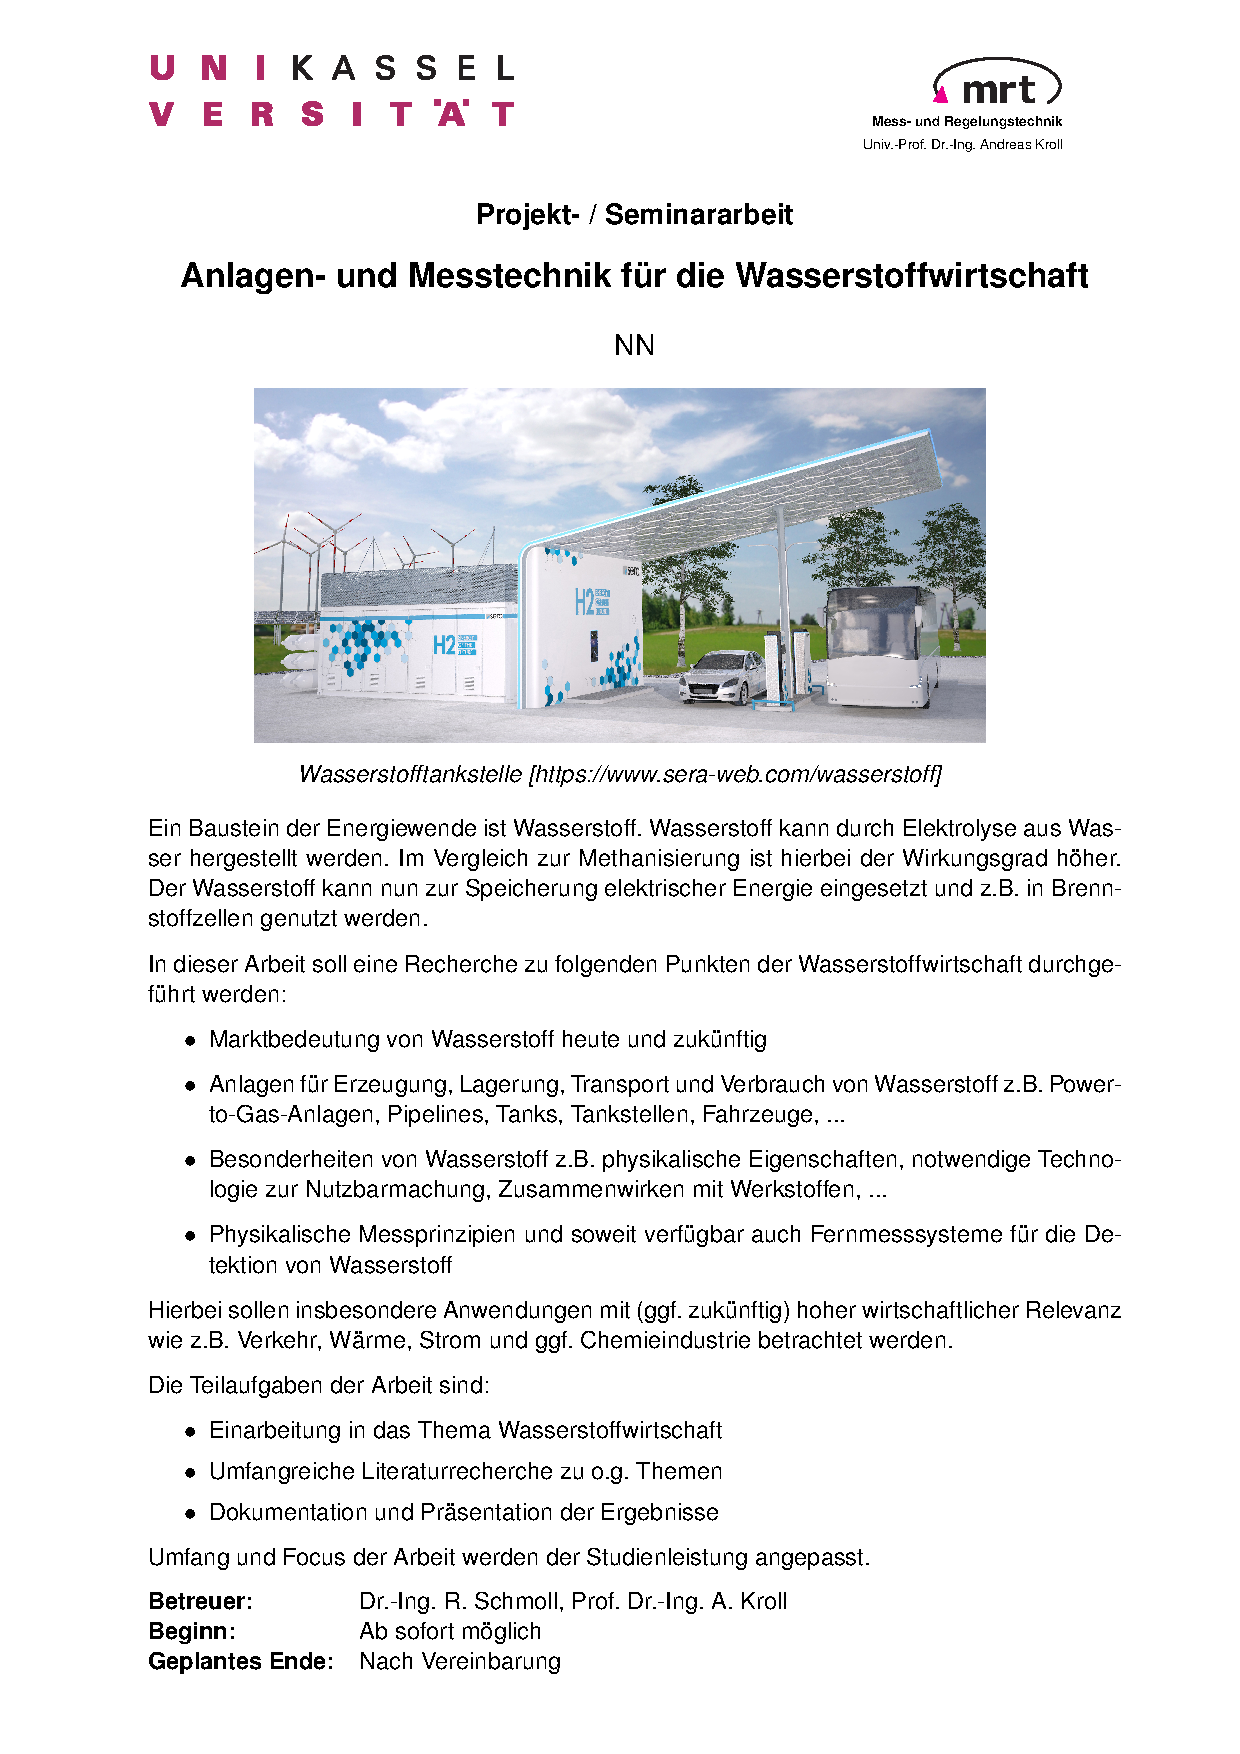
\includegraphics[width=1.0\textwidth,page=1]{\Aufgabenstellung}}
\end{figure}

\begin{figure}[!htbp]
\centering
\fbox{\includegraphics[width=1.0\textwidth,page=2]{\Aufgabenstellung}}
\end{figure}
\cleardoublepage
}{}

% --------------------------------------------------------------------------
% Versicherung (BEI BA UND MA)
% --------------------------------------------------------------------------
\ifthenelse{\equal{\Typ}{MSc}\or\equal{\Typ}{BSc}}{
% !TeX encoding = UTF-8
% !TeX TS-program = pdflatex
% !TeX spellcheck = de_DE

\chapter*{Versicherung}

Hiermit versichere ich, dass ich die vorliegende Arbeit selbstständig
verfasst und keine anderen als die angegebenen Quellen und Hilfsmittel
verwendet habe.

\vspace*{5ex}
\rule{12cm}{0.5pt}\newline
Ort, Datum, Unterschrift


%%% Local Variables:
%%% mode: latex
%%% TeX-master: "../MRT-Bericht2020"
%%% End:

\cleardoublepage
}{}

% --------------------------------------------------------------------------
% Zusammenfassung (BEI BA UND MA)
% --------------------------------------------------------------------------
\ifthenelse{\equal{\Typ}{MSc}\or\equal{\Typ}{BSc}}{
% !TeX spellcheck = de_DE
\chapter*{Kurzfassung}

Hier das Interesse des Lesers wecken!

Warum soll er diese -- genau diese -- Arbeit lesen?


\ifthenelse{\equal{\Typ}{MSc}}{
\vfill
\section*{Summary}
\begin{otherlanguage}{english}
Awaken the reader's interest here!

Why should he read this - exactly this - work?
\end{otherlanguage}

\selectlanguage{ngerman}
}{}

%%% Local Variables:
%%% mode: latex
%%% TeX-master: "../MRT-Bericht-2020"
%%% End:

\cleardoublepage
}{}

% --------------------------------------------------------------------------
% Summary (BEI MA)
% --------------------------------------------------------------------------
%\ifthenelse{\equal{\Typ}{MSc}}{
%\include{Kapitel/Summary}
%\cleardoublepage
%}{}

% --------------------------------------------------------------------------
% Inhaltsverzeichnis (IMMER)
% --------------------------------------------------------------------------
\tableofcontents
\cleardoublepage

% --------------------------------------------------------------------------
% Liste der Tabellen und Bilder und Listings
% --------------------------------------------------------------------------
\listoftables      % optional
\listoffigures     % optional
\lstlistoflistings % optional
\cleardoublepage

% --------------------------------------------------------------------------
% Abkürzungsverzeichnis (IMMER)
% --------------------------------------------------------------------------
% !TeX spellcheck = de_DE
\chapter*{Abkürzungsverzeichnis}
\addcontentsline{toc}{chapter}{Abkürzungsverzeichnis}

\begin{center}
	
	\renewcommand{\arraystretch}{1.1}
	\tablefirsthead{\hline \textbf{Abkürzung} & \textbf{Bedeutung} \\ \hline}
	\tablehead{\hline \textbf{Abkürzung} & \textbf{Bedeutung} \\ \hline}
	
	\begin{supertabular}{p{2.1cm}p{10.9cm}}
		API				& \textbf{A}pplication \textbf{P}rogramming \textbf{I}nterface \\
		GigE			& \textbf{G}igabit \textbf{E}thernet \\
		PoE				& \textbf{P}ower \textbf{o}ver \textbf{E}thernet \\
		GUI				& \textbf{G}raphical \textbf{U}ser \textbf{I}nterface \\
		UML				& \textbf{U}nified \textbf{M}odeling \textbf{L}anguage \\
		MES				& \textbf{M}anufacturing \textbf{E}xecuting \textbf{S}ystem\\
		C\#				& An object oriented, component oriented programming language\\
		C++				& A high level, general purpose programming language\\
		QML				& \textbf{Q}t-Project's Interface \textbf{M}arkup \textbf{L}anguage\\
		LZ				& \textbf{L}ager\textbf{zelle} der $\mu$Plant\\
		FZ				& \textbf{F}ertigungs\textbf{zelle} der $\mu$Plant \\
		AuE				& \textbf{A}bfüll- \textbf{u}nd \textbf{E}ntleer - Station der $\mu$Plant \\
		RFID			& \textbf{R}adio \textbf{F}requency \textbf{ID}entification\\
		TCP/IP			& \textbf{T}ransmission \textbf{C}ontrol \textbf{P}rotocoll / \textbf{I}nternet \textbf{P}rotocoll\\
		MVC				& \textbf{M}odel - \textbf{V}iew - \textbf{C}ontroller, Ein Design-Konzept für Software\\
		URI				& \textbf{U}niform \textbf{R}essource \textbf{I}dentifier, Im Qt Framework kann dies eine beliebige
						  Ressource sein. Z.B. eine URL, ein Bild oder ein Programmteil. \\
		QML Type		& Ein QML Basiselement. Enthält alle für die Visualisierung nötigen Attribute. Eine Liste
						  aller QML Types findet sich hier \cite{qmlTypeList}\\
		RAPID			& Eine speziell für die Robotersteuerung entwickelte Programmiersprache\\
		RST				& \textbf{R}e\textbf{s}tructured \textbf{T}ext Eine einfache markup language die in Sphinx benutzt wird\\
	\end{supertabular}

\end{center}
\addcontentsline{toc}{chapter}{Abkürzungsverzeichnis}
\printglossary[title={Abkürzungsverzeichnis},toctitle={Abkürzungsverzeichnis}]
\cleardoublepage

% --------------------------------------------------------------------------
% Symbolverzeichnis (IMMER)
% --------------------------------------------------------------------------
%% !TeX spellcheck = de_DE
\chapter*{Symbolverzeichnis}
\addcontentsline{toc}{chapter}{Symbolverzeichnis}

\begin{center}
	
	\renewcommand{\arraystretch}{1.1}
	\tablefirsthead{\hline \textbf{Symbol} & \textbf{Beschreibung} & \textbf{Einheit} \\ \hline}
	\tablehead{\hline \textbf{Symbol} & \textbf{Beschreibung} & \textbf{Einheit} \\ \hline}
	
	\begin{supertabular}{p{1.85cm}p{9cm}p{1.85cm}} % GESAMT 12.7cm!
		% Latein: Alphabetisch + 1. Matrizen, 2. Großbuchstaben, 3. Vektoren, 4. Kleinbuchstaben
		$\varepsilon$ 	& Emissionsgrad 	& - \\
	\end{supertabular}

\end{center}
\addcontentsline{toc}{chapter}{Symbolverzeichnis}
\printnomenclature
\cleardoublepage

% --------------------------------------------------------------------------
% Index (optional)
% --------------------------------------------------------------------------
\addcontentsline{toc}{chapter}{Index}
\printindex
\cleardoublepage


% --------------------------------------------------------------------------
% Hauptteil der Arbeit (IMMER)
% --------------------------------------------------------------------------
\pagestyle{fancy2}
\setcounter{SeitenzahlSpeicher}{\value{page}}
\pagenumbering{arabic}

% Erklärung gemäß Prüfungsordnung
% Danksagung

% !TeX encoding = UTF-8
% !TeX TS-program = pdflatex
% !TeX spellcheck = de_DE

\chapter{Motivation und Zielsetzung}

    Das Institut für Mess- und Regelungstechnik an der Universität Kassel hat in den letzten Jahren eine Modellfabrik $\mu$Plant gebaut.
    Aus über 70 Einzelarbeiten ist ein modernes Industrie-4.0 Konzept geschaffen worden.
    Teil der $\mu$Plant ist ein vollautomatisiertes Lager.
    Das Lager besteht aus einem abgetrennten Raum, dessen Zugang über eine Tür mit einem Türschalter überwacht ist.
    In diesen Bereich können autonome mobile Roboter (Turtlebots) einfahren.
    In dem abgetrennten Bereich steht ein Industrieroboter Typ ABB IRB 140 und ein Lagerregal mit ausgewiesenen 18 Lagerplätzen.
    Außerdem befindet sich neben einer Andockstation für den Turtlebot ein Kommissioniertisch. \\

    Ein pneumatischer Greifer kann Paletten, die je mit bis zu zwei Bechern bestückt werden können,
    zwischen dem mobilen Roboter und dem Lagerregal transportieren.
    Von einem PC-Arbeitsplatz aus können mittels Software die Lagerprozesse überwacht werden.
    Im Fehlerfall kann eingeschritten werden oder es können manuell Prozesse ausgelöst werden.\\

    Die Software ist derzeit in 3 Programme aufgeteilt: Einerseits gibt es die Lagerverwaltung 3.0 - die Hauptsoftware.
    Sie bildet die automatisierten Prozesse ab und verfügt über ein GUI welches u.A.\ den Bestand visualisiert.
    Daneben gibt es den Warehouse Controller, der dazu verwendet wird, manuelle Prozesse auszulösen.
    Zudem gibt es ein Programm \glqq RFID-Server\grqq mit dem über RFID Leser der Fa. Feig Tags der Transportbehälter
    ausgelesen werden können.
    \\
    Mit dem Wechsel des Betriebssystems von Windows 7 auf Windows 10 ist die Kompatibilität der C\# Implementierung
    nicht mehr gegeben.
    Außerdem laufen Teilfunktionen des Programms nicht fehlerfrei oder tolerieren kaum Fehlbedienungen.
    Die Dreiteilung der Software ist im Allgemeinen auch nicht mehr erwünscht. \\

    Diese Seminararbeit beschäftigt sich mit der Analyse der bestehenden Software:
    Es wird ermittelt, aus welchen Programmteilen und Funktionen die Software besteht.
    Aus den Erkenntnissen wird ein Konzept entwickelt, welches die Funktionen der Drei Software Teile zusammenführt.
    Dies soll die Grundlage für eine Migration der Software nach Python schaffen.

    Erkenntnisse aus der studentischen Arbeit von Sebastian Hübler aus dem Jahr 2019 \cite{Hübler2019} sollen überprüft
    und vertieft werden um Anforderungen an Kameras und arUco Marker zu ermitteln, die später eine automatisierte
    Inventur ermöglichen sollen.


\cleardoublepage

\chapter{Kurzbeschreibung der Lagerzelle}\label{Lagerzelle}

    Die Lagerzelle ist ein abgesperrter Bereich innerhalb der $\mu$Plant. 
    Sie hat eine überwachte Zugangstür für Personen und eine Andockstation für einen mobilen Roboter, die für Personen nicht passierbar ist. 
    Die Andockstation ist mit einem RFID-Lesegerät der Fa. FEIG GmbH und zwei induktiven Näherungssensoren ausgestattet, sowie einer 
    Ladestation. 
    
    Direkt dahinter steht ein ABB Industrieroboter IRB 140 auf seinem Fundament. 

    Aus Sicht des Roboters um $90^\circ$ dazu befindet sich ein Kommissionier-Tisch mit Platz für bis zu zwei Paletten.
    Die Paletten-Plätze sind mit \glqq K1\grqq{} und \glqq K2\grqq{} gekennzeichnet.
    Für die Becher sind die Plätze \glqq a\grqq{} und \glqq b\grqq{} auf der vom Roboterarm abgewandten Seitde des Tisches
    angebracht.

    Wiederum $90^\circ$ versetzt zum Kommissioniertisch, also gegenüber der Andockstation befindet sich ein Lagerregal.
    Es hat drei Böden mit jeweils sechs Lagerplätzen für Paletten.
    Die Lagerplätze sind mit \glqq L1\grqq{}(oben links) bis \glqq L18\grqq{}(unten rechts) gekennzeichnet.
    An der dem Benutzer zugewandten Seite sind die Becherplätze \glqq a\grqq{}(vorne) und \glqq b\grqq{}(hinten) angebracht.
    
    Der Roboterarm hat einen pneumatischen Greifer, mit dem er eine Palette oder einen Becher aufnehmen kann. 
\cleardoublepage

\chapter{Softwarearchitekturanalyse bestehender Programme}\label{SoftwareArchitektur}

    Analysemethoden der Informatik für Software sind in der Regel für die verschiedenen Design-Phasen entwickelt worden.
    Eine von mir durchgeführte Internet-Recherche ergab, dass sich Analyse-Tools und Methoden für bestehende Software vor
    allem darauf fokussieren, die Performance, Speichermanagement und Benutzererfahrung zu bewerten.
    Die Architektur einer Software spielt dabei eine untergeordnete Rolle.
    Für einen Nachfolger der Lagerverwaltung 3.0 soll jedoch zunächst ihre Softwarearchitektur untersucht werden.
    Die Performance und der Speicherverbrauch spielen für die $\mu$Plant eine untergeordnete Rolle.
    Eine Bewertung der Programmkomponenten sollt also anhand folgender Kriterien bewertet werden:

    \begin{itemize}
        \item Ihrem Nutzen für den Anwender
        \item Zuverlässigkeit im Betrieb
        \item Umgang mit erwartbaren Fehlern
    \end{itemize}

    Der Programmcode sollte zudem
    \begin{itemize}
        \item Leicht lesbar und verständlich,
        \item Zuverlässig und robust, und
        \item gut erweiterbar sein.
    \end{itemize}
    In einem C$\#$ Projekt sind GUI und Buisinesslogik in getrennten Dateien implementiert.
    XAML-Dateien gehören zu Microsofts .NET Plattform. 
    Ihr Dateiformat ähnelt denen von XML-Dateien. 
    Sie legen fest wie das GUI gerendert wird und werden im integrierten Editor der Visual Studio IDE bearbeitet.
    .XAML.cs Dateien implementieren die Controller-Logik des XAML-Inhalts. 
    Ihre Programmiersprache ist C$\#$.

    Am Beispiel des Startbildschirms des Programms \glqq Lagerverwaltung 3.0\grqq wird der Programmaufbau geschildert.
    Aufgrund der Komplexität und des fehlenden Mehrwerts wird weiteren Verlauf dieser Arbeit darauf verzichtet.
    Aus dem gleichem Grund wird auf die detaillierte Beschreibung der Funktionsweise von grafischen ELementen ihrer Events
    sowie ihrer Eventhandler verzichtet.

    In den erstellen Klassendiagrammen ist gut ersichtlich, welche Klassen Events nutzen.
    Sie erben von der Klasse \verb|INotifyPropertyChanged|.
    Die Klasse ist ein Interface der .NET Plattform und wird immer dann eingesetzt, wenn eine GUI-Komponente über eine Änderung
    informiert werden soll. Sie wird im Allgemeinen dafür benutzt um das GUI mit dem hinterlegten Datenmodell zu verknüpfen.

    Wenn diese Klasse implementiert wird, muss die Methode \verb|OnPropertyChanged| überschrieben werden, die immer dann aufgerufen wird,
    wenn sich ein Wert ändert. 
    \clearpage

    \section {Lagerverwaltung 3.0}

    Wie in dem einleitenden Abschnitt angekündigt wird zunächst der grundlegende Aufbau des Programms beschrieben.\\

    Die Datei \verb|App.xaml| ist der Einstiegspunkt des Programms.
    In ihr wird ein Objekt der Application-Klasse mit allen benötigten Ressourcen erzeugt.
    Als Start URL ist \verb|MainWindow.xaml| angeben.\\
    In der Datei ist beschrieben, wie der Startbildschirm gerendert wird.

    Zunächst wird ein Banner gerendert, bestehend aus dem Titel des Programms, dem Logo des Instituts und der $\mu$Plant
    (Siehe Abb.\ref{fig:figure} Bereich \glqq A\grqq).
    Es werden außerdem alle benötigten Datenobjekte erzeugt.
    Sie lassen sich wie folgt einteilen:
    
    \begin{itemize}
        \item Objekte und Variablen, die dem Lager zugeordnet sind:
            \begin{itemize}
                \item Ein Objekt \verb|inventory| der Klasse \verb|Inventory| für das Inventar mit \verb|null| initialisiert.
                \item Ein Objekt \verb|storageMatrix| von der Klasse \verb|PalletMatrix| erzeugt.
                \item Ein Object \verb|commissionMatrix| von der Klasse \verb|PalletMatrix| erzeugt.
                \item Ein Objekt \verb|mobileRobot| von der Klasse \verb |MobileRobot| erzeugt.
                \item Außerdem eine Variable \verb|lastCupRead| vom Datentyp \verb|ushort| (16-Bit-Ganzzahl, vorzeichenlos) mit 0 initialisiert.
            \end{itemize}
            \item Objekte und Variablen initialisiert, die dem ABB Controller zugeordnet sind:
            \begin{itemize}
                \item Ein Objekt \verb|commands| von der Klasse \verb|controllerCommandList|.
                \item Ein Objekt \verb|controllerProperties| von der Klasse \verb|RobotControllerProperties|.
                \item Ein Objekt \verb|controllerBase| von der Klasse \verb|RobotControllerBas|, mit dem Initialisierungswert \verb|null|.
                \item Ein Objekt \verb|controllerSim| von der Klasse \verb|RobotSimulator|.
            \end{itemize}
    \end{itemize}

    Im Constructor der Klasse \verb|MainWindow| werden zudem der ModBus und der Roboter Controller initialisiert
    und ihre GUI-Elemente gerendert (Abb.\ref{fig:figure} Bereiche \glqq B\grqq{} und \glqq C\grqq).
    
    Die Produktliste wird aus der Datei \verb|Produkte.db| geladen und gerendert (Abb.\ref{fig:figure} Bereich \glqq D\grqq).
    
    Daten des Lagers und des mobilen Roboters sowie die Kommissionsdaten werden aus der Datei \verb|CommissionData.db|
    geladen und anschließend das Inventar gerendert (Abb.\ref{fig:figure} Bereich \glqq E\grqq{}  und \glqq G\grqq).
    
    Bereich \glqq F\grqq{} ist der Eventlog der Anwendung, dort werden alle Ereignisse der Software als Text angezeigt.
    Das können Fehler sein aber auch Fortschritte im Programmablauf.

    Im mittleren Bereich ist die Anordnung von Roboter, Andockstation und Kommissioniertisch symbolisiert.
    Der \glqq Start\grqq -Knopf startet den Automatikbetrieb.
    Nach dem Start der Automatik kann der selbe Knopf zum Stoppen des Automatikbetriebs verwendet werden.

    Wenn keine Verbindung zum Modbus hergestellt werden kann, wird dem Benutzer angeboten die Vorgänge zu simulieren.
    Im Klassendiagramm Abb.\ref{fig:figure2} wird jedoch schnell deutlich, dass dieser Simulationsbetrieb nicht für einen Testbetrieb
    geeignet ist, da dazu eine ganz andere Klasse verwendet wird.

    Im Bereich \glqq Mobile Robot\grqq{} wird nach erfolgreichem Andocken das erkannte Produkt angezeigt.
    Dem Bediener wird hier angeboten die Daten manuell zu manipulieren oder Details ein- bzw. auszublenden.

    Im Bereich \glqq Workbench\grqq{} werden bis zu zwei Paletten mit ihrem Inhalt gerendert.
    Auch hier wird dem Benutzer angeboten, die Daten per Hand zu manipulieren.

    Im Folgenden werden die wichtigsten Klassenstrukturen beschrieben.
    Auf die Beschreibungen von Hilfsklassen und solche, die für die .NET Plattform oder die Programmiersprache C$\#$ spezifisch sind, wird verzichtet.

    \begin{figure}[h]
        \caption[Ansicht des Startbildschirms]
        {\small Startbildschirm der Anwendung, zur besseren Beschreibung sind die Bedienbereiche rot umrandet und mit
        Buchstanben gekennzeichnet}\label{fig:figure}
        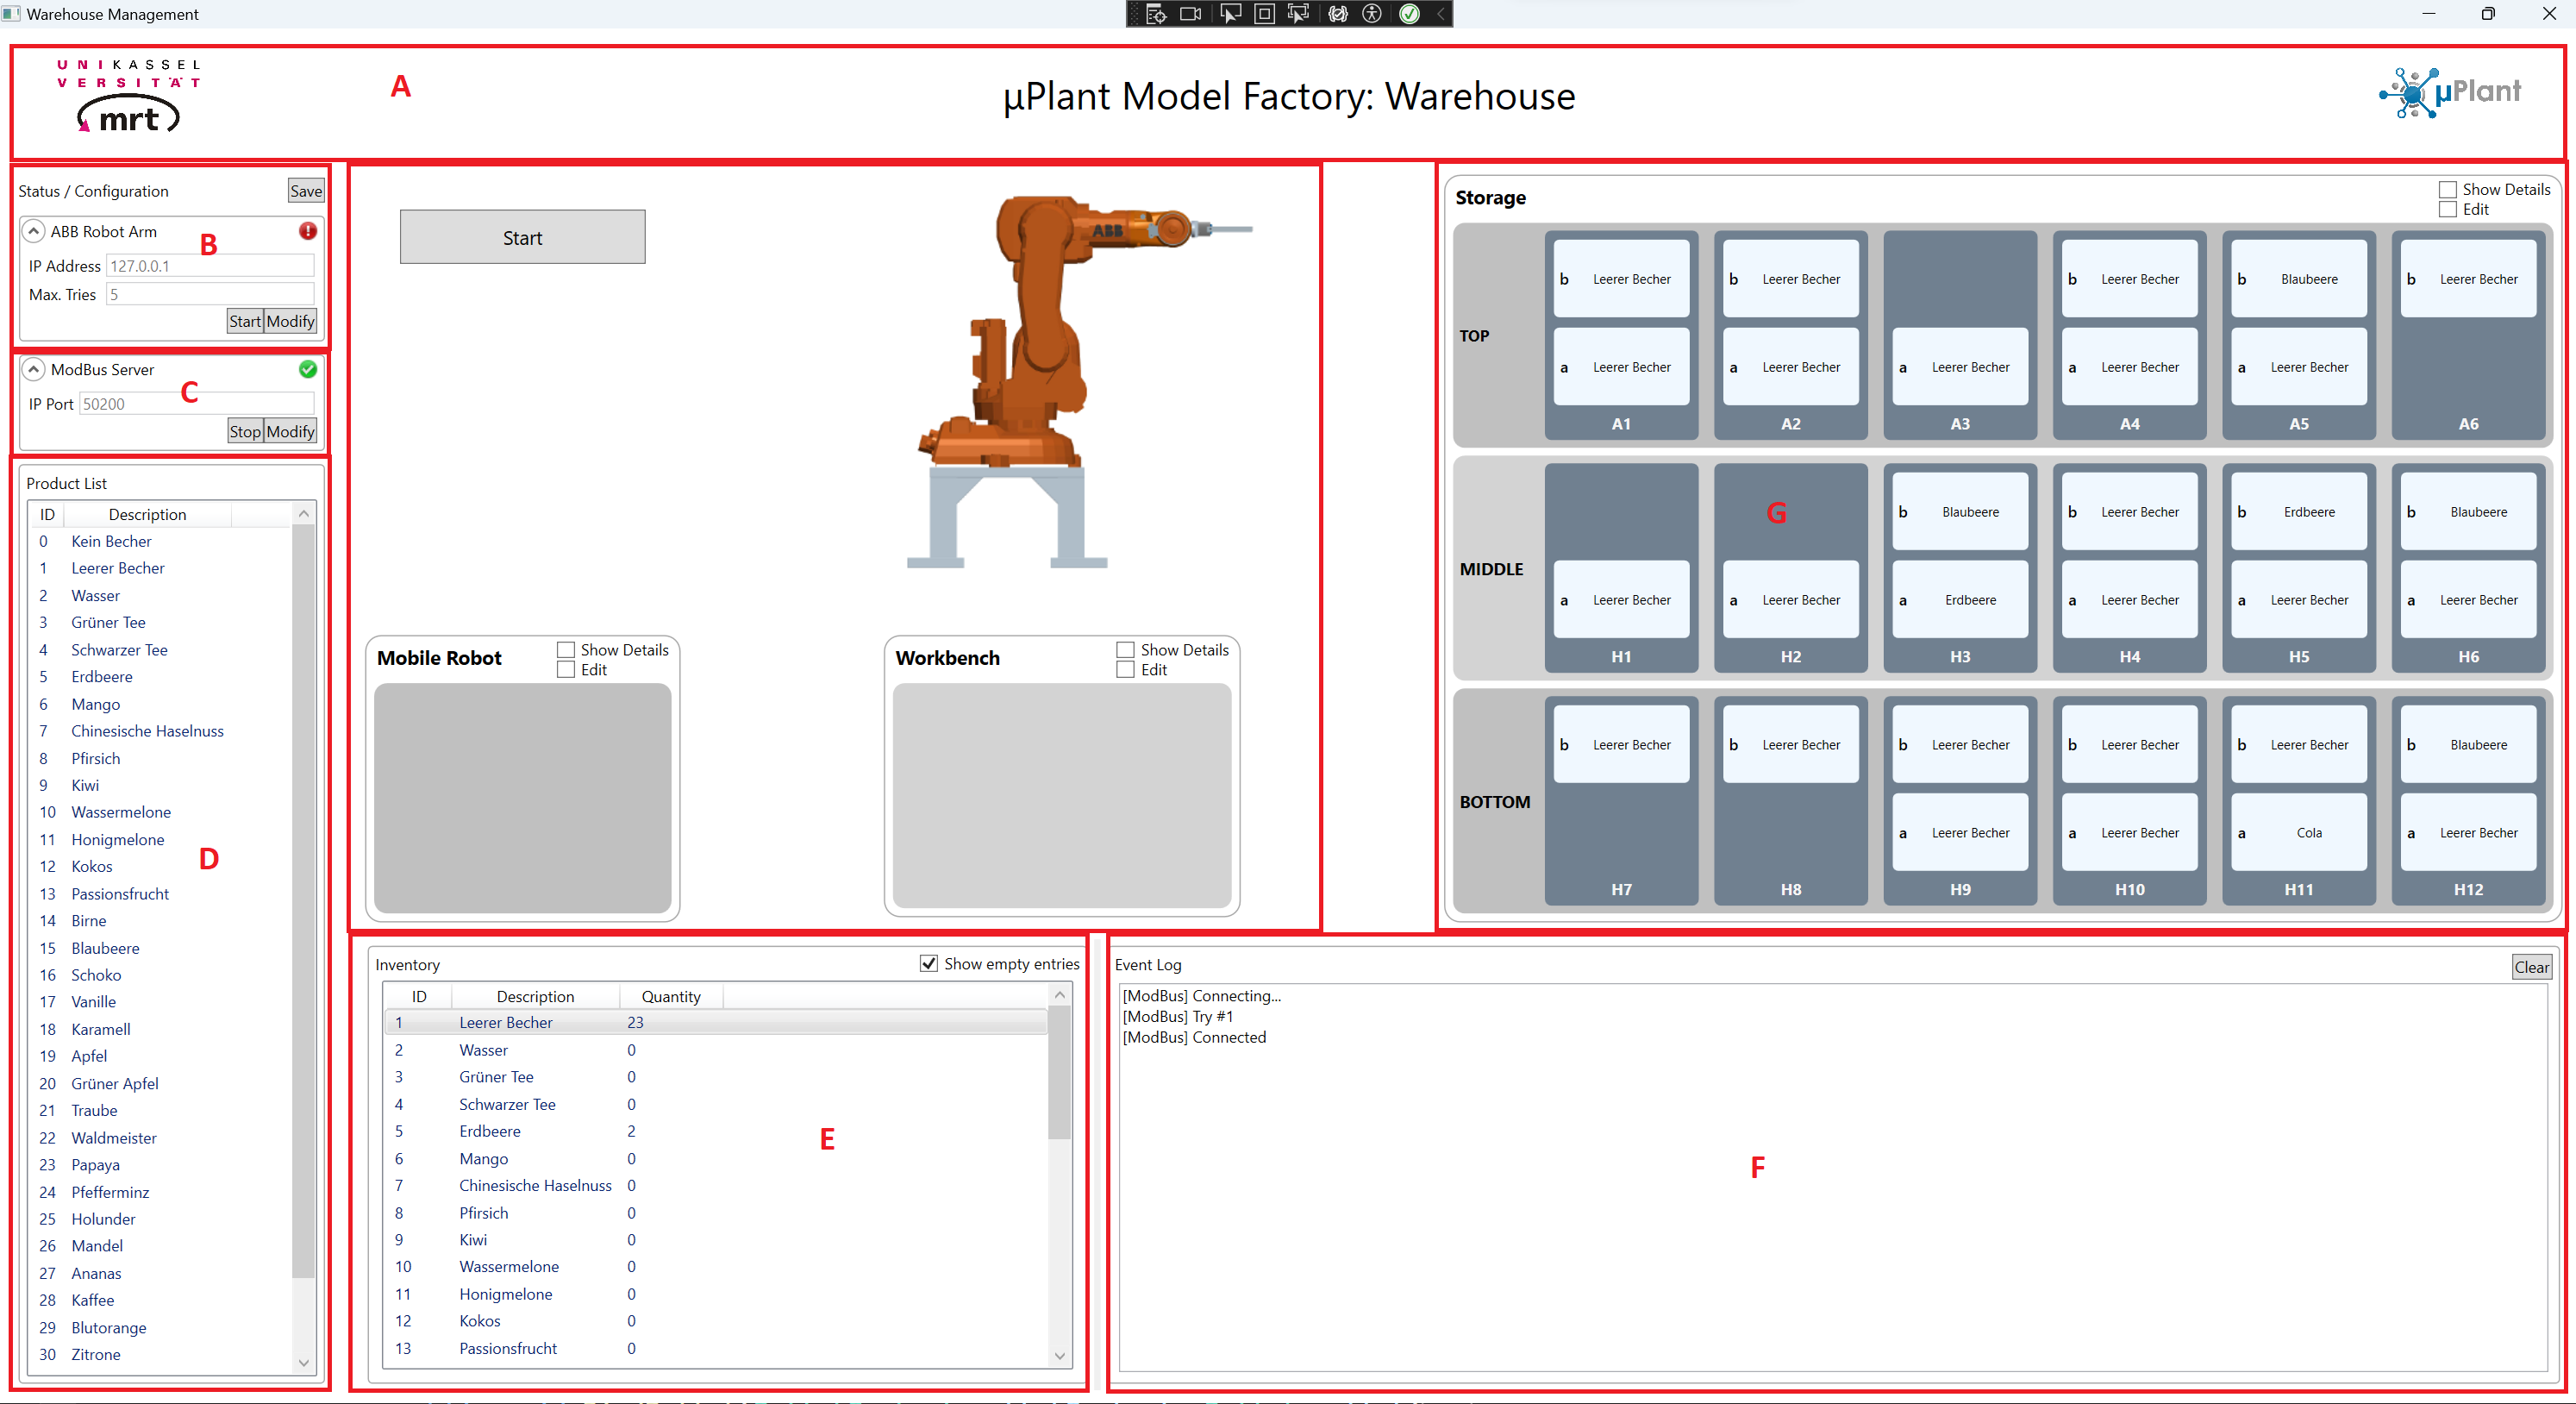
\includegraphics[width = \textwidth ]{Bilder/LV_Startbildschirm}
        \centering
    \end{figure}

    \subsection{Klassenstruktur des Datenmodells}\label{Datenmodell}

    Die bestehende Software dient dazu Lagerpakete vom mobilen Roboter auf die Werkbank oder ins Lager zu bewegen.
    Oder alle möglichen Kombinationen davon. 
    Ein Lagerpaket ist einer der nachfolgenden Varianten:
    \begin{itemize}
        \item Ein Becher
        \item Eine leere Palette
        \item eine Palette mit einem oder zwei Bechern
    \end{itemize}
    
    Der Programmierer hat sich diese Struktur angeeignet und in der Datenmodellierung umgesetzt.
    In Abb.\ref{fig:figure2} ist gut ersichtlich, dass die Klasse \verb|StorageElementBase| an die Klassen \verb|Cup| und \verb|Pallet|
    vererbt (schmale Linie mit leerem Pfeil, in Anlehnung an UML). Eigenschaften, die sowohl Palette als auch den
    Becher betreffen, sind in dieser Klasse implementiert.

    Weiterhin findet sich das Lager als eigene Klasse \verb|Inventory| und der mobile Roboter als \verb|MobileRobot| wieder.
    Die \verb|Inventory|-Klasse ist jedoch nicht das Lager im Sinne von Abb.\ref{fig:figure2} Bereich \glqq G\grqq, sondern auf die Liste in
    Bereich \glqq E\grqq.\\

    \begin{figure}
        \caption[Klassendiagramm Datenmodells ]
        {\small Klassendiagramm der MainWindow-Klasse mit vererbenden- und Datenmodell - Klassen }\label{fig:figure2}
        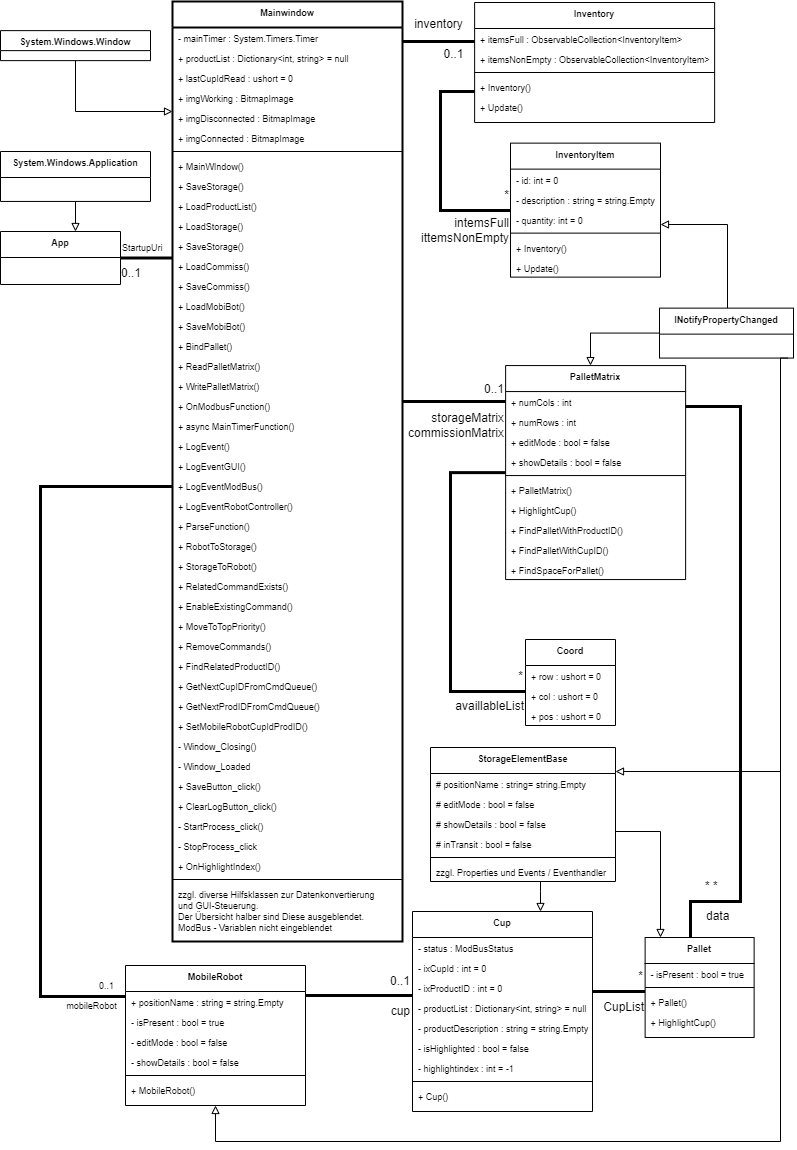
\includegraphics[width = \textwidth ]{Bilder/LV_Klassendiagramm_Datenmodell}
        \centering
    \end{figure}
    \clearpage

    Zentrales Element ist die \verb|MainWindow| Klasse.
    Sie implementiert eigentlich die Interface-Klasse \verb|System.Windows.Window|.
    Der Programmierer hat sie allerdings auch als Daten-Hub verwendet.
    
    Wie zu Beginn des Abschnitts geschildert werden beim Rendern des Fensters alle benötigten Datenobjekte erzeugt oder aus Dateien geladen.

    \begin{itemize}
        \item In der Klasse \verb|Inventory| wird der Inhalt der Datei \verb|Produkte.db| in zwei Listen geladen, sodass
        eine Liste mit lagernden Produkten und eine vollständige Produktliste gespeichert werden.
        Eine Instanz \verb|inventory| wird zur Laufzeit erzeugt. Wenn die Dateien \verb|Produkte.db| und
        \verb|StorageData.db| zu dem Zeitpunkt nicht verfügbar ist, stürzt das Programm ab.
        \item In der Klasse \verb|PalletMatrix| wird die Datei \verb|StorageData.db| bzw. \\ \verb|CommissionData.db|
        geladen um einen zweidimensionalen Array \verb|data| zu erzeugen.
        Jedes Array-Element ist ein Objekt der Klasse \verb|Pallet| und enthält eine Liste \verb|CupList| von Objekten
        der Klasse \verb|Cup|.
        Diese Struktur wird dazu verwendet, um das reale Lager zu visualisieren.
        Zur Laufzeit werden zwei Objekte der Klasse \verb|PalletMatrix| erzeugt:
        \begin{itemize}
            \item \verb|storageMatrix| bildet das Datenmodell um die Visualisierung in Abb.\ref{fig:figure2} Bereich \grqq G\glqq{} zu realisieren.
            \item \verb|commissionMatrix| bildet das DatenModell für die Visualisierung des mobilen Roboters und der
            Workbench.
        \end{itemize}
    \end{itemize}
\newpage
    \begin{figure}
        \caption[Klassendiagramm ABBRobotics Controller ]
        {\small Klassendiagramm der MainWindow-Klasse mit Klassen aus dem ABBRobotics Controllerframework. }\label{fig:figure3}
        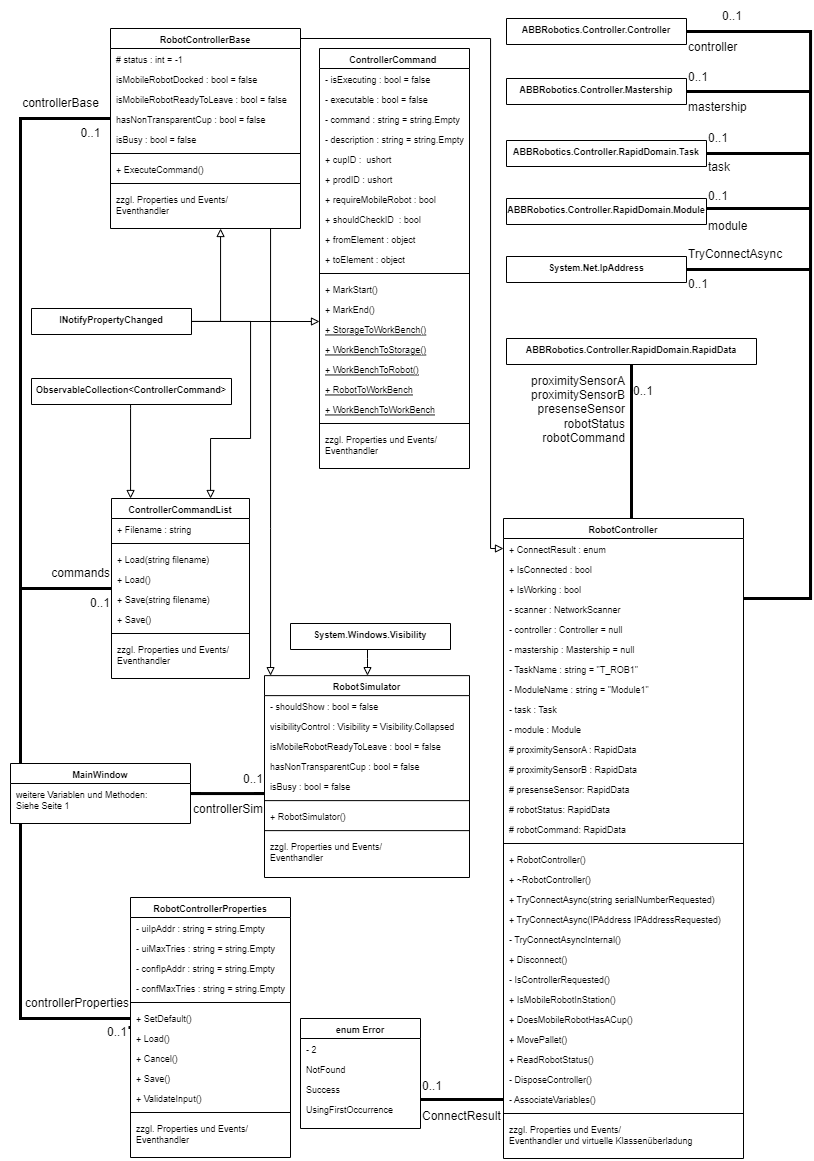
\includegraphics[width = \textwidth ]{Bilder/LV_Klassendiagramm_ABBController}
        \centering
    \end{figure}

\subsection{Klassenstruktur zur Steuerung des ABB Industrieoboter IRB 140}\label{ABBKlassen}

Um dem Industrieroboter ABB IRB 140 Kommandos zu senden, muss das Programm mit der Steuerung IRC5 kommunizieren.
Die Steuerung ist Baujahr 1991 und hat eine Firmware \glqq RobotWare 5.15.1004.01\grqq{} installiert.
Die Kommunikation erfolgt über ein verschlüsseltes TCP/IP Protokoll. 

Im Programmcode finden sich dazu wie in Abb.\ref{fig:figure3} gezeigt, die Klassen der Bibliothek \verb|ABBRobotics|.
Instanzen dieser Bibliothekbestandteile werden in der Klasse\\ \verb|RobotController| erzeugt, die von der Klasse
RobotControllerBase erbt.

Interessant ist, dass in der \verb|MainWindow| Klasse kein Objekt von RobotController erzeugt wird, sondern eiens von der Klasse
\verb|RobotControllerBase| \glqq controllerBase\grqq{}, welches mit \verb|null| initialisiert wird. 
Diese Klasse hat Properties für die Näherungssensoren der Andockstation und virtuelle Funktionen um den Status abzurufen, 
den mobilen Roboter als abfahrbereit zu melden und Kommandos auszuführen. 

In der Methode \verb|StartProcess_click| - also mit Klick auf den Start Button - wird das Objekt verändert mit der Zuweisung

$$controllerBase = robotControl.controlHandler;$$

Die Zuweisung löst die Anmeldung des PC's mit der Steuerung aus und gibt als Rückgabewert ein Objekt der Klasse \verb|RobotController| zurück. 

\subsubsection{Klassen und Methoden der Kommandos}

Die Klasse \verb|ControllerCommandList| erbt von einer Liste der Klasse\\ 
\verb|ControllerCommand|.  Beide Klassen gehören zum namespace der 
\verb|RobotControllerBase|.

Beim Initialisieren des Programms wird eine leere \verb|ControllerCommandlist| erzeugt. 
Die Klasse \verb|ControllerCommand| hat Properties, die bspw. den Status, ein Kommando-Datenstring und eine Beschreibung des Kommandos enthalten. 
Sie implementiert demnach das Datenmodell der Kommandos. 

Die Methoden und Variablen in der Klasse implizieren, dass die Commands aus einer Datei geladen werden.
Sie lassen sich aber sowohl in der IDE Visual Studio als auch in der IDE Rider keine Verweise zu den Methoden finden.

Die Klasse ControllerCommand hat 5 statische Methoden.
Jede von ihnen gibt ein Objekt der Klasse \verb|ControllerCommand| zurück.
\begin{itemize}
    \item \verb|StorageToWorkBench| übermittelt der Steuerung den Befehl eine Palette vom Lager zum Kommissioniertisch
    zu transportieren.
    \item \verb|WorkBenchToStorage| übermittelt der steuerung den Befehl eine Palette vom Kommissioniertisch zum Lager
    zu transportieren.
    \item \verb|WorkBenchToRobot| übermittelt der Steuerung den Befehl eine Palette vom Kommissioniertisch auf den
    mobilen Roboter zu platzieren.
    \item \verb|RobotToWorkBench| übermittelt der Steuerung den Befehl eine Palette vom mobilen Roboter auf den
    Kommissioniertisch zu transportieren.
    \item \verb|WorkBenchToWorkBench| übermittelt der Steuerung den Befehl, dass eine Palette den Platz auf dem
    Kommissioniertisch wechseln soll.

\end{itemize}
Als Parameter in der Methodensignatur werden die Koordinaten der Start- und Endpunkte übergeben
sowie \verb|Pallet| Objekte am Start- und Endpunkt.

In dem ControllerCommand Objekt werden zwei Strings erzeugt, die am Beispiel\\
\verb|StorageToWorkBench| erklärt werden:
\newline
\lstinputlisting[language = Python, caption = Formatierung eines Kommandos an den IRB140 Roboterarm, label=command ]{Listings/commandFormat.cs}

\verb|station| ist ein Integer mit dem Wert von 3, wenn die oberste Regalreihe ausgewählt wurde, oder 2 sonst.

\verb|position| ist ein Integer, der sich aus der Spalte des Lagerregals errechnet.

\verb|w_col+1| ist die Angabe des Ortes am Kommissioniertischs.


\lstinputlisting[language = Python, caption = Erzeugung eines beschreibenden Strings für den Eventlog, label=commandDsc ]{Listings/commandDescription.cs}


Mit \ref{commandDsc} wird ein String erzeugt, der eine Beschreibung des Vorgangs enthält.\\
Die \verb|ControllerCommands| werden in Methoden der \verb|MainWindow| Klasse erzeugt.
Die Parameter der Funktionssignatur stammen aus dem Objekt \verb|commissionMatrix| welche in Kapitel \ref{Datenmodell}
bereits beschrieben wurde.

Die \verb|MainWindow| Klasse hat eine Timer-gesteuerte Funktion \verb|MainTimerFunction|, die die Commands
fallweise abarbeitet.
Wie genau die Daten vom Modbus Server in die \verb|commissionMatrix| geschrieben werden konnte ich mit meinen eher
bescheidenen C$\#$ Kenntnissen nicht ermitteln.
\newpage

\subsection{Klassenstruktur Modbus TCP/IP}\label{ModbusChapter}

Modbus ist ein open-source Kommunikationsprotokoll welches 1979 von Modicon (heute Schneider Electric) veröffentlicht wurde.
Es wird dazu verwendet Client-Server Verbindungen einzurichten und ist laut Modbus Organization de facto Standard in
industriellen Herstellungsprozessen.
Modbus unterstützt verschiedene Kommunikationsstrukturen.
Modbus TCP/IP ist lediglich eine Variante, die 1999 entwickelt und veröffentlicht wurde.
TCP/IP ist das übliche Transportprotokoll des Internets und besteht aus einer Reihe von Layer Protokollen, die einen
zuverlässigen Datentransport zwischen Maschinen bereitstellen.
Die Verwendung von Ethernet TCP/IP in der Fabrik ermöglicht eine echte Integration mit dem Unternehmensintranet und
MES-Systemen, die die Fabrik unterstützen.
Die Protokollspezifikation und Implementierungsanleitung sind auf der Seite der Modbus Organization frei verfügbar\cite{ModbusOrg}.
\newline
\newline
Lars Kistner \cite{LarsKistner2017} hat in seiner Bachelorarbeit aus dem Jahr 2016 die Kommunikationsstruktur der $\mu$Plant
festgelegt.
Wie er beschreibt, existiert ein zentraler Modbus Server, der die \glqq Kommandos\grqq in die entsprechenden Modbus
Adressen und/oder Funktionsregister schreibt.
Diese Adressen sind in der Datei \verb|ModbusBaseAddress.cs| niedergeschrieben und und um die Adressen des mobilen Roboters
ergänzt.
\begin{table}[h]
\centering
\caption{Werte der Klasse ModbusBaseAddress}
\begin{tabular}{|l|l|c|}
\hline
Adresse & Wert & Beschreibung \\
\hline
Status & 1 & \\
\hline
KeepAlive & 2 &\\
\hline
Working & 3 &\\
\hline
FunctionReady & 5 &\\
\hline
ResponseReady & 6 &\\
\hline
Done & 7 &\\
\hline
AgentLockID & 8 &\\
\hline
AgentLockRequest & 9 &\\
\hline
FunctionID & 10 &\\
\hline
FunctionParameters & 11 &\\
\hline
FunctionParametersLength & 32 &\\
\hline
ResponseID & 43 &\\
\hline
ResponseParameters & 44 &\\
\hline
ResponseParametersLength & 32 &\\
\hline
StorageCup & 1024 &\\
\hline
StorageProduct & 1280& /// 1024 + 256\\
\hline
CommissionCup & 2048 &\\
\hline
CommissionProduct & 2080 & /// 2048 + 32\\
\hline
MobileRobotCup & 2560 &\\
\hline
MobileRobotProduct & 2568 & /// 2560+8\\
\hline
MobileRobotDocked & 2576 &\\
\hline
MobileRobotReadyToLeave & 2580 &\\
\hline
\end{tabular}\label{tab:ModbusBase}
\end{table}


\clearpage
Schaut man sich das Klassendiagramm der Modbus - Implementierung \ref{fig:figure4} an, stellt man fest, dass es die Klasse
\verb|MainWindow| Objekte von drei verschiedenen Klassen instanziiert, die sich dem Modbus Protokoll zuordnen lassen.

Sie besitzt ein Objekt der Klasse \verb|ModbusStatus| welches ein Objekt der Klasse \\\verb|ModBusCommunication| besitzt.

\verb|modbusTCP.modbusTCPServer| wird ebenfalls als Objekt in \verb|MainWindow| erzeugt.
Gleichzeitig wird sie aber auch in \verb|ModbusCommunication| instanziiert.

Die dritte Klasse ist \verb|ModbusProperties|.
Sie ist eine Datenklasse und enthält die IP-Adresse und den Port des Modbus Servers.

\verb|CommissionMatrix|
Die Klasse RobotController übersetzt diese in Strings und schickt sie an die IRC5 Steuerung.
Wenn diese den Befehl ausgeführt hat, meldet sie \glqq Fertig\grqq{} zurück.

Im Anhang B.5 seiner Arbeit sind die Modbus-Adressen, die dem Lager zugeordnet sind, aufgelistet.
Der Adressenbereich ist lückenlos zwischen 1024 und 1105.
Jeder Ablageort eines Bechers (z.B. L1a für Lagerort L1, vorne) hat zwei Adressen: Eine für die Cup ID und eine
für die Product ID.
Das schließt den Kommissioniertisch und den mobilen Roboter mit ein.

\begin{figure}
    \caption[Klassendiagramm Modbus ]
    {\small Klassendiagramm der MainWindow-Klasse mit Mosbus-Klassen }\label{fig:figure4}
    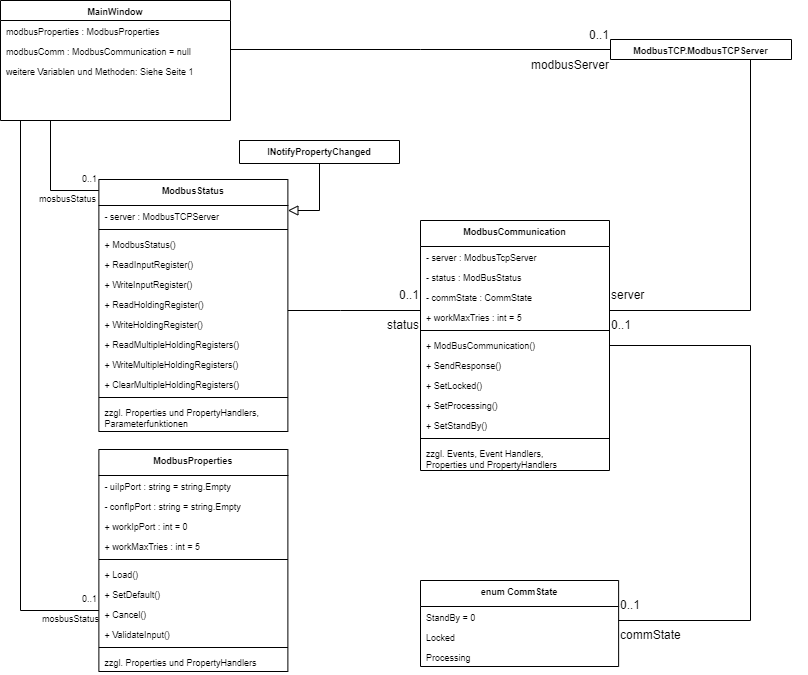
\includegraphics[width = \textwidth ]{Bilder/LV_Klassendiagramm_Modbus}
    \centering
\end{figure}

\subsection{GUI}
Das GUI besteht aus einem Fenster, welches in 8 Bereiche unterteilt ist (siehe Abb.\ref{fig:figure}).
Der Bereich \glqq A\grqq{} hat keine Bedienfunktion.

\subsubsection{ABB Controller Einstellungen}

Der Bereich \glqq B\grqq{} ermöglicht dem Benutzer die Verbindungsdaten zur Steuerung des ABB Roboter IRB140 zu
konfigurieren und die Verbindung herzustellen. 
Die Verbindungsdaten sind voreingestellt und die Felder sind standardmäßig für die Eingabe deaktiviert. 
Die Aktivierung des Felds erfolgt über die Taste \glqq Modify\grqq{}.
Mit der Taste \glqq Save\grqq{} können Änderungen gespeichert werden.

Mit der \glqq Start\grqq{} Taste wird die Verbindung hergestellt.
Die Taste verändert daraufhin ihren Text zu \glqq Connecting...\grqq{} und bei erfolgreich hergestellter Verbindung
zu \glqq Stop\grqq{}.
Ein Symbolbild Informiert dabei über den Verbindungsstatus.

\subsubsection{Modbus Einstellungen}
Im Bereich \glqq C\grqq{} kann der IP-Port des Modbus-Servers über die Taste \glqq Modify\grqq{} angepasst werden.
Direkt nach Programmstart, noch vor der Betätigung der Start-Taste, ist das Symbolbild für den Verbindungsstatus grün
und suggeriert eine erfolgreiche Verbindungsherstellung. 
Nach meinem Verständnis handelt es sich hierbei um eine Fehl-Initialisierung.

Die Verbindungstaste zum Starten der des Automatikbetrieb steht zum Programmstart auf \glqq Stop\grqq{}.

\subsubsection{Produktliste}
Im Bereich \glqq D\grqq{} befindet sich eine scrollbare Liste aller möglichen Produkte mit zwei Spalten.
Es wird neben dem Produktnamen die Produkt-ID angezeigt.
Vermutlich dient die Liste als Nachschlagewerk oder Übersicht, denn es sind ansonsten keine Bedienfunktionen verfügbar.

\subsubsection{Inventaranzeige}
Im Bereich \glqq E\grqq{} Ist die Gleiche Liste um eine Spalte erweitert, in der die gelagerte Menge aufgeführt ist.
Die Liste bildet somit eine bessere Übersicht über das gelagerte Inventar und ist auch als \glqq Inventory\grqq{} gekennzeichnet.
Mit der Checkbox \glqq Show empty entries\grqq{} können Produkte ohne eingelagerte Menge ausgeblendet werden.

\subsubsection{Eventloganzeige}
Bereich \glqq F\grqq{} ist ein Eventlog. Hier werden von dem Programm aus verschiedenste Mitteilungen dem Benutzer angezeigt.
Mit der Taste \glqq clear\grqq{} werden alle existierenden Einträge gelöscht.

\subsubsection{Lagervisualisierung}
Bereich \glqq G\grqq{} ist die Visualisierung des Lagers.
Die drei Reihen \glqq TOP\grqq{}, \glqq MIDDLE\grqq{} und \glqq BOTTOM\grqq{} sollen die drei Regalböden des Lagerregals nachbilden.
Sie sind als hellgraues Rechteck gerendert.

Die Slots A1\ldots A6, H1\ldots H6 sowie H7\ldots H12 sind die Plätze für je eine Palette, die wiederum Platz für
je zwei Becher hat.
Der Ursprung dieser Bezeichnung konnte während der Vorbereitungen auf diese Arbeit nicht geklärt werden.
Wie ich in \ref{Lagerzelle} beschriebe habe, weicht diese Art der Bezeichnung der Lagerplätze von der realen lagerzelle ab.

Das dunkelgraue Rechteck mit der Beschriftung des Lagerorts symbolisiert die Palette.
Die beiden weißen Rechtecke darauf symbolisieren je einen Becher.
Sie sind mit \glqq a\grqq{} für vorne und \glqq b\grqq{} für hinten gekennzeichnet und zeigen den Produktnamen an.

Ist ein Slot für einen Becher leer, wird das entsprechende Rechteck nicht gerendert.
Ein leerer Becher ist ein Produkt im Sinne des Programms.

Ist keine Palette vorhanden, verbleibt der gesamte Bereich der Palette leer.

In der oberen, rechten Ecke kann der Benutzer mit der Checkbox \glqq Show Details\grqq{} zusätzlich die Becher-ID und die
Produkt-ID ein- und ausblenden.

Mit der Checkbox \glqq Edit\grqq{} kann der Benutzer alle Daten (Palette vorhanden/ nicht vorhanden, Becher-ID, Produkt-ID)
als Eingabefeld sehen und ändern.
Der Produktname wird dabei über die Produkt-ID referenziert.
Die Änderungen werden gespeichert, indem die Checkbox einfach wieder abgewählt wird.

\subsubsection{Prozessvisualisierung}

Der Bereich der Prozessvisualisierung ist in der Mitte des Bildschirms.

Im Automatikbetrieb ist dieser grob in 4 Bereiche eingeteilt. 

\textbf{Oben Rechts} ist ein Symbolbild des Industrieroboters IRB 140 dargestellt. 
Das Bild bietet keinerlei Bedienfunktion.

\textbf{Oben links} befindet sich die Start-Taste und im Simulationsbetrieb weitere GUI-Elemente.
Wenn die Verbindungen zum Modbus und zur IRC5-Steuerung hergestellt sind, kann mit ihr der Automatikbetrieb gestartet werden.
Ist der Modbus nicht verbunden, erscheint nach dem Klick ein Dialogfenster.
Der Benutzer wird gefragt, ob aufgrund der fehlenden Verbindung der Controller simuliert werden soll.
Klickt man nun auf \glqq Ja\grqq{}, wird über dem mobilen Roboter ein weiteres Rechteck gerendert.
Es enthält zwei Checkboxen \glqq Mobile Robot is present\grqq{} und \glqq Robot has non-transparent cup\grqq{}.
Erstere rendert nach dem Klick einen mobilen Roboter (schwarzes Oval) und gibt dem Benutzer die Möglichkeit,
wie gewohnt über die beiden Checkboxen im oberen rechten Bereich, Daten eines Bechers und Produkts einzugeben.
Klickt man nun wieder auf die Taste, die nun mit \glqq Stop\grqq{} beschriftet ist, erscheint für etwa eine Sekunde
der Schriftzug \glqq Wait...\grqq{}, bevor das Programm wieder in den Ausgangszustand wechselt.

\textbf{Unten links} befindet sich die Visualisierung des mobilen Roboters. 

\textbf{Unten rechts} befindet sich die Visualisierung des Kommissioniertischs.

Beide Lagerbereiche, für den mobilen Roboter und den Kommissioniertisch,  
geben dem Benutzer die Möglichkeit die Becher- bzw. Produkt-ID ein- und auszublenden oder zu überschreiben.

Weiterhin bietet das Programm keine Möglichkeit den Roboter zu steuern.

\clearpage
\section {Controller}

Der Controller ist eine kleine Anwendung, die die manuelle Bedienung der Lagerzelle ermöglicht.
Die Implementierung der RFID - Funktionen können anhand des Klassendiagramms nicht gezeigt werden.
In Vorbereitung auf diese Arbeit habe ich nicht ausprobiert, ob das Programm diese Funktionen so erfüllt wie sie in dem
GUI impliziert wird.
Für die weitere Arbeit würde dies auch keinen Mehrwert bieten, wie sich in Kapitel \ref{PythonApp}
noch zeigen wird.

\subsection{Klassenstruktur des Controllers}

Der Controller ist genau wie die Lagerverwaltung 3.0 in C$\#$ zusammen mit der .NET-Plattform implementiert.
Da der Controller keinen eigenen Modbus-Server hostet sondern die Klasse \verb|ModbusClient| nutzt, kann er ohne die 
Anwendung \glqq Lagerverwaltung 3.0\grqq{} nicht benutzt werden.

In Abb.\ref{fig:figure6} sieht man, dass das Programm aus zwei wesentlichen Klassen neben dem \verb|MainWindow| besteht.
\verb|ModbusClient| implementiert den Modbus Clienten zur Kommunikation mit den Modbus Servern, die in \ref{ModbusChapter}
beschrieben sind. Die Klasse implementiert auch das in \cite{LarsKistner2017} beschriebene Agentensystem.
\verb|ModbusInfo| dagegen hält die Daten, die zur Erzeugung der Kommandos benötigt werden.

Mit dem Konstruktor der Klasse \verb|MainWindow| werden die Klassen \verb|ModbusClient| und \verb|ModbusInfo| instanziiert.

\begin{figure}
    \caption[Klassendiagramm des Controllers]
    {\small Klassendiagramm des Controllers mit allen vererbenden Klassen, jedoch ohne Klassen die
    lediglich Datentypen konvertieren.}\label{fig:figure6}
    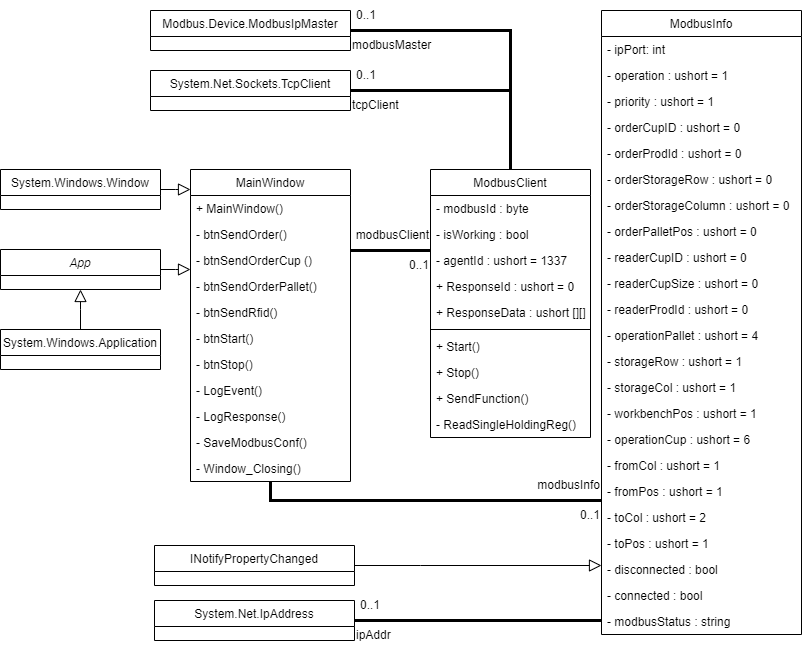
\includegraphics[width = \textwidth ]{Bilder/C_Klassendiagramm}
    \centering
\end{figure}


\subsection{GUI}

\begin{figure}
    \caption[Ansicht des Controller- Startbildschirm ]
    {\small Ansicht des Controller Startbildschirms. }\label{fig:figure5}
    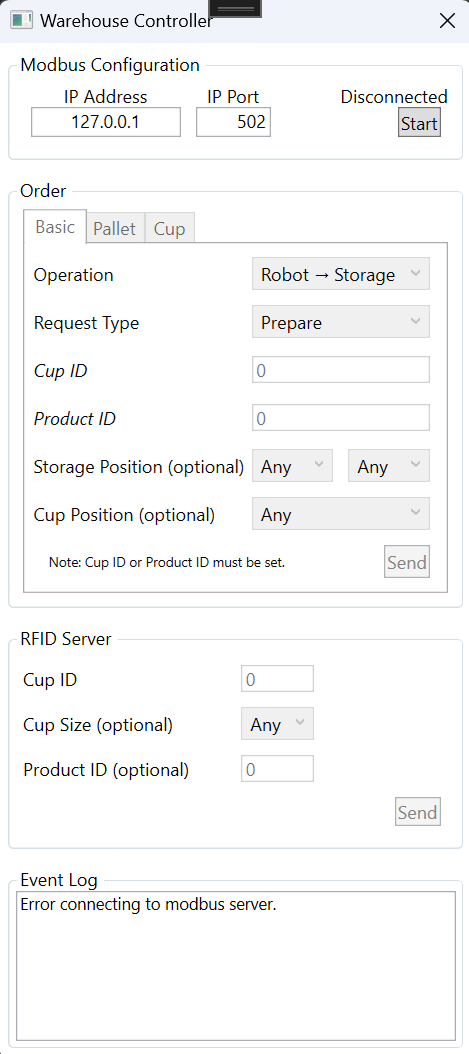
\includegraphics[height = \textheight ]{Bilder/Controller_Startbildschirm}
    \centering
\end{figure}

Wie in \ref{fig:figure5} ersichtlich, ist das Fenster einfach strukturiert und übersichtlich.
Es ist in vier Bereiche unterteilt, die durch eine grau umrandete Box und eine Überschrift abgegrenzt sind.

\subsubsection{Modbus Einstellungen}

Dieser Bereich ist ganz oben und durch die Überschrift \glqq Modbus Configuration\grqq{} gekennzeichnet.
In zwei Textfeldern können Modbus-IP und -Port eingegeben werden. 

Rechts daneben befinden sich untereinander zum Einen ein Label, dass den Verbindungsstatus anzeigt und zum Anderen
ein Knopf mit dem die Verbindung hergestellt und beendet werden kann.

Nach dem Programmstart ist die Beschriftung der Taste \glqq Start\grqq{}.

Mit Klick auf die Taste wird die Verbindung hergestellt und das Label darüber wechselt zu \glqq Connecting...\grqq{}.
Ist die Verbindung erfolgreich hergestellt, wechselt das Label auf \glqq Connected\grqq{} und die Taste wird mit
\glqq Stop\grqq{} beschriftet.

\subsubsection{Kommando erzeugen}

Direkt unter dem Modbus Einstellungsbereich befindet sich der Bereich \glqq Order\grqq{}.
Der Bereich ist durch ein Reitermenü ausgefüllt, dessen Reiter die Überschriften
\glqq Basic\grqq{}, \glqq Pallet\grqq{} und \glqq Cup\grqq{} tragen.

Im Reiter \glqq Basic\grqq{} befinden sich sieben Auswahlfelder und eine Taste.

Mit dem Feld \glqq Operation\grqq{} kann über ein Drop-Down Menü ausgewählt werden, ob ein Becher oder Produkt vom Roboter ins Lager transportiert werden soll oder umgekehrt.

Mit dem Feld \glqq Request Type\grqq{} kann über ein Drop-Down Menü ausgewählt werden, ob der Transport nur Vorbereitet (\glqq Prepare\grqq{}) oder auch ausgeführt (\glqq Execute\grqq{}) werden soll.

Darunter befinden sich Eingabefelder über die die relevante ID (Becher oder Produkt) eingegeben werden kann.

Optional kann darunter über ein Drop-Down Menü die Lagerposition des Lagers oder Bechers ausgewählt werden.


Mit der Taste \glqq Send\grqq{} wird das Kommando an die Steuerung gesendet.

Im Reiter \glqq Pallet\grqq{} kann analog der Transport einer Palette angefordert werden.

Im Reiter \glqq Cup\grqq{} kann analog der Transport eines Bechers angefordert werden.

\subsubsection{RFID Server Tool}

Mit dem RFID Server Tool, dargestellt unter dem Reitermenü, können Speicherblöcke eines RFID-Tags mit der Becher-ID und/oder Produkt-ID
beschrieben werden.
Voraussetzung dafür ist, dass der mobile Roboter mit Becher in der Andockstation des steht.

Die IDs werden in einem Eingabefeld als Zahl eingegeben. Optional kann die Bechergröße ausgewählt werden. 

Mit der Taste \glqq Send\grqq{} werden die Daten auf das RFID-Tag geschrieben.

\subsubsection{Eventlog}

Dies ist ein Textbereich in dem die angeforderten Kommandos aufgelistet werden und eine Mitteilung wenn sie erfolgreich ausgeführt wurden.


\clearpage
\section {RFID Server}

Dieses kleine Programm implementiert einen Modbus TCP/IP Client wie in \ref{ModbusChapter} beschrieben.
Dieser wird genutzt um die gelesenen RFID-Tags für alle Stationen der $\mu$Plant verfügbar zu machen.

In jeder Station der $\mu$Plant gibt es einen RFID Leser der Fa. Feig.

Stationen in der $\mu$Plant können einen Tag am Becher beschreiben wenn sie das Produkt im Becher manipulieren oder die Tags auslesen.
Anschließend können Stationen die einen Becher erhalten, den angekündigten Becher und das Produkt beim Eintreffen
in der Station verifizieren.
Die Verfahren dazu sind in \cite{LarsKistner2017} gut beschrieben.

Die Daten der Tags sollen beim Schreiben und Lesen auf die Modbus Adressen des Modbus Servers geschrieben werden.

Die Auftragswervaltung der $\mu$Plant kann die Daten der Tags dann vom Modbus Server abrufen.
Die RFID-Lesegeräte werden über TCP/IP mittels des SDK der Fa. Feig angesprochen.

\subsection{Klassenstruktur des RFID Servers}

\begin{figure}
    \caption[Klassendiagramm des Programms RFID Server ]
    {\small Klassendiagramm des Programms RFID Server mit allen vererbenden Klassen jedoch ohne solche die
    lediglich Typen konvertieren.}\label{fig:figure8}
    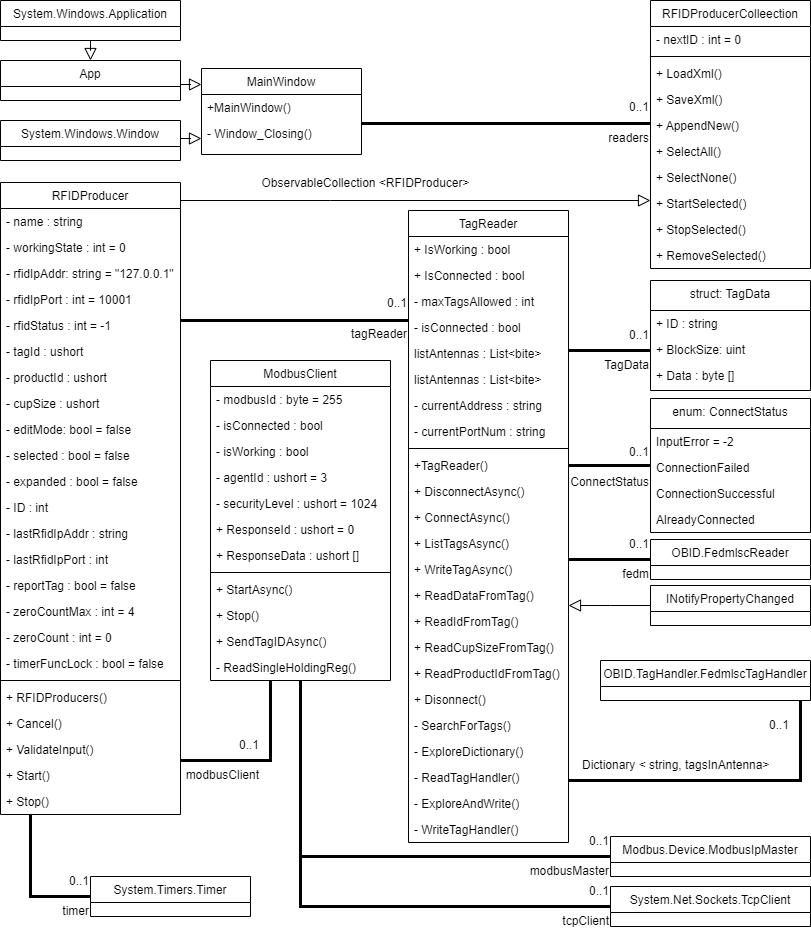
\includegraphics[width = \textwidth ]{Bilder/RFID_Klassendiagramm}
    \centering
\end{figure}

Die Programmstruktur ist anhand des Klassendiagramms in \ref{fig:figure8} erklärt.
Eine Klasse \verb|MainWindow| hält eine Instanz der Klasse \verb|RFIDProducerCollection|.

Diese implementiert die oben beschriebene Liste welche Objekte der Klasse \verb|RFIDProducer| speichert.

Ein \verb|RFIDProducer| Objekt enthält ein Objekt der Klasse \verb|ModbusClient| für die Kommunikation über TCP/IP und
ein Objekt der Klasse \verb|TagReader| für die RFID Kommunikation.


\subsection{GUI}
Das GUI des RFID-Servers ist einfach gehalten und ist in Abb.\ref{fig:figure7} dargestellt.
Das Hauptelement ist eine Liste.
Jedes Listenelement enthält Daten zu einem RFID Modbus Server und einem Tag mit seinen Daten.
Mit der Taste \glqq Add New\grqq{} können neue, leere, Listenelemente erzeugt werden.

Standardmäßig sind die Eingabefelder deaktiviert, können jedoch mit der Taste \glqq Modify\grqq{} zum Bearbeiten
freigeschaltet werden.

Mit der Taste \glqq Start\grqq{} wird die Verbindung hergestellt. Ein Feedback, ob die Verbindung erfolgreich hergestellt
werden konnte ist zunächst nicht ersichtlich.

Jedes Listenelement enthält eine Checkbox mit der es ausgewählt werden kann.

Mit den Tasten \glqq Select All\grqq{} und \glqq Select None\grqq{} können alle Listenelemente an- oder abgewählt werden.

Im unteren, rechten Bereich können mit den Tasten \glqq Start Selected\grqq{} und \glqq Stop Selected\grqq{} mehrere Server
gleichzeitig gestartet und gestoppt werden.

Mit der Taste \glqq Remove Selected\grqq{} können alle ausgewählten Listenelemente gelöscht werden.

\begin{figure}
    \caption[Startbildschirm des Programms RFID-Server]
    {\small Startbildschirm des Programms RFID-Server}\label{fig:figure7}
    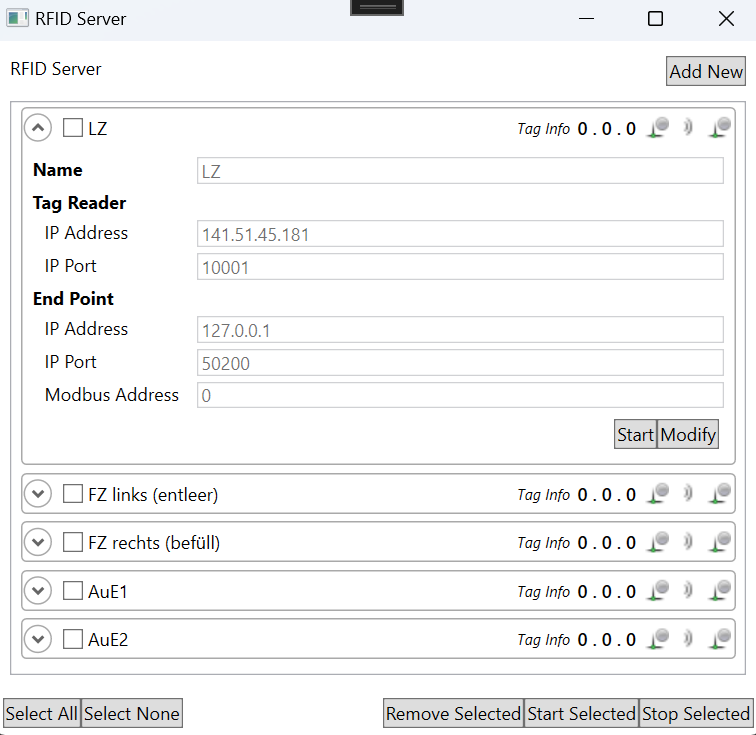
\includegraphics[height = \textwidth ]{Bilder/RFIDServer_Bildschirm}
    \centering
\end{figure}

\cleardoublepage

\chapter{Funktions- und Anforderungsanalyse}\label{Funktionsanalyse}

In diesem Kapitel werden auf Grundlage der vorangegangenen Kapitel die notwendigen Funktionen und ihre Anforderungen ermittelt. 
Der daraus entstehende Funktions- und Anforderungsumfang dient als Grundlage für das Kapitel \ref{PythonApp}.

\section{Lagerverwaltung 3.0}
Dieses Programm hat ein Anwendungsfenster welches dem Benutzer einen umfassenden Überblick über die LZ gibt.

Das Fenster hat eine Mindest- und Maximalgröße, ist dazwischen aber beliebig skalierbar. 

Dialoge werden genutzt, wenn Einträge gelöscht werden, Verbindungen nicht aufgebaut werden könenn und der Simulationsbetrieb gestartet werden kann.

Felder sind standardmäßig deaktiviert und müssen über Checkboxen aktiviert werden. 

Dateneingaben erfolgen über Dropdown Menüs wenn eine Auswahl festgelegter Werte möglich ist. 
Ansonsten werden Eingabefelder benutzt.

\subsection{Bedienfunktionen}

Der Benutzer kann über das GUI folgende Eingriffe vornehmen:

\begin{itemize}
    \item Die Verbindung zu einem Modbus Server konfigurieren, starten und beenden.
    \item Die Verbindung zur ABB IRC5 Steuerung konfigurieren, speichern, starten und beenden.
    \item In der Produktliste kann gescrollt werden.
    \item In der Inventarliste kann gescrollt werden und es können leere Produkte ein- und ausgeblendet werden.
    \item Die vergangenen Einträge im Eventlogger können gelöscht werden. Im Eventlogger kann gescrollt werden.
    \item In der Lagervisualisierung können an den einzelnen Lagerorten
    \begin{itemize}
        \item Paletten hinzugefügt oder entfernt werden
        \item Becher hinzugefügt oder entfernt werden
        \item Produkt ID und Cup ID der Becher können angezeigt und konfiguriert werden
        \item Durch Klick auf einen Becher werden alle Becher gleichen Produkts in der Lagervisualisierung und auch im
        Inventar blau hervorgehoben.
    \end{itemize}
    \item Palette, Becher und Produkt auf dem Kommissioniertisch können konfiguriert werden
    \item Becher und Produkt auf dem mobilen Roboter können konfiguriert werden.
    \item Der Automatikbetrieb kann gestartet werden
    \item Wenn die Verbindung zum Modbus Server nicht hergestellt wurde kann ein Simulationsbetrieb gestartet werden
    \item Im Simulationsbetrieb kann zudem
    \begin{itemize}
        \item Die Anwesenheit eines mobilen Roboters Simuliert werden
        \item ausgewählt werden, dass der Becher auf dem mobilen Roboter nicht transparent ist (Funktion unklar)
    \end{itemize}
\end{itemize}

\subsection{Informationsdarstellung}

Der Benutzer wird über folgende Inhalte informiert:

\begin{itemize}
    \item Die Verbindungseinstellungen des Modbus Servers und den Verbindungsstatus
    \item Die Verbindungseinstellungen des ABB-Controllers und ihren Verbindungsstatus
    \item Alle möglichen Produkt ID's und die zugehörigen Produktnamen
    \item Produkte und ihre Lagermengen im Inventarbereich.
    \item In der Lagervisualisierung:
    \begin{itemize}
        \item Symbolisierung einer Palette durch dunkelgraues Rechteck, wenn eine Palette vorhanden ist
        \item Symbolisierung der Becher durch weißes Rechteck, wenn ein Becher vorhanden ist
        \item Produknamen und auf Wunsch auch Produkt ID und Becher ID
    \end{itemize}
    \item Im Eventlogger werden folgende Informationen bereit gestellt:
    \begin{itemize}
        \item Fehler und Events der Verbindung über Modbus TCP/IP
        \item Fehler und Events der Verbindung zur Steuerung IRC5 des Industrieroboters
        \item Programmfortschritte und Events im Automatikbetrieb oder der Simulation
    \end{itemize}
\end{itemize}

\section{Controller}

Der Benutzer kann folgende Bedienvorgänge durchführen:

\begin{itemize}
    \item Die Verbindungseinstellungen des Modbus Servers konfigurieren und starten
    \item Transportbefehle können erzeugt werden:
    \begin{itemize}
        \item Transportbefehle eines einzelnen Bechers zwischen Lager, Kommissioniertisch und Roboter
        \item Transportbefehle für einer Palette zwischen Lager und Kommissioniertisch
    \end{itemize}
    Die beiden Befehle können einerseits direkt ausgeführt werden, andererseits können sie auch als Eingabe für die
    Lagerverwaltungssoftware benutzt werden.
    \item Ein Becher in der Andockstation kann mittels einem RFID- Lesegerät beschrieben werden.
\end{itemize}

Der Benutzer wird in diesem Programm nur über seine Eingaben Informiert.
Die Eingaben erfolgen wo möglich über ein Dropdown Menü

\section{RFID Server}

Der Benutzer kann folgende Bedienvorgänge durchführen:

\begin{itemize}
    \item Einen Neuen Listeneintrag erzeugen
    \item Einen oder alle Listeneintrag markieren
    \item Markierte Listeneinträge abwählen
    \item ausgewählte Listeneinträge Löschen, Verbindung starten oder stoppen
    \item Je Listeneintrag kann der Benutzer folgende Einstellungen vornehmen:
    \begin{itemize}
        \item IP und Port des Tag Readers
        \item IP, Port und Modbus Adresse des Endpoints
    \end{itemize}
    \item Ein einzelner Listeneintrag kann gestartet werden
    \item Mit der Taste \glqq Modify \grqq kann ein Listeneintrag zum Bearbeiten freigeschaltet werden
    \item Mit der Taste \glqq Save \grqq können Änderungen gespeichert werden.
\end{itemize}

Der Benutzer sieht in diesem Programme eine Liste aller eingetragenen RFID Reader, Endpoints und Modbus Adressen.
Jeder Listeneintrag kann auf eine Zeile minimiert werden die lediglich den Namen des Endpunkts und die gelesenen
Tag Daten anzeigt.
Im ausgeklappten Zustand sind die Konfigurationen sichtbar, aber grau hinterlegt um anzudeuten, dass die Bearbeitung
gesperrt ist.



\cleardoublepage


\chapter{Konzeptionierung einer integrierten Python Anwendung}\label{PythonApp}

Die Basisanforderungen einer integrierten LZ-Verwaltung lassen sich aus Kapitel \ref{Kap2} ableiten.
Hinzu kommen die später in Kapitel 5 beschriebenen Funktionen.
Neben den Kriterien Modularität, Erweiterbarkeit und Wartbarkeit ist darüber hinaus wichtig, dass auch Personen,
die bei der ursprünglichen Entwicklung der Software nicht involviert waren die Software warten und weiterentwickeln können.
Eine saubere Struktur der Software ist daher unerlässlich und impliziert eine objektorientierte Programmierung.
Die alte Software nutzte eine GUI-Klasse als Datenhub.
Dadurch entstand ein unübersichtliches Klassenkonstrukt, dass es schwer machte den Code zu überschauen.
Zum Beispiel wird anhand der Klassendiagramme deutlich, dass Daten der Modbus Adressen in die \verb|commissionMatrix|
geschrieben werden müssen, weil sie ausschließlich dort zu RAPID Kommandos für den Industrieroboter übersetzt werden.
Wie genau das passiert, lässt sich jedoch anhand des C\# Codes nicht nachvollziehen.
Mit genügend Zeitaufwand könnte dieses Rätsel aufgelöst werden, jedoch bringt es für die Konzeptionierung der neuen
Software keinen Mehrwert.\\
\vspace{1cm}
Um den genannten Anforderungen gerecht zu werden, empfiehlt es sich auf branchenübliche Design Patterns
zurückzugreifen.
Das MVC Konzept sieht vor, dass Daten (Model) und GUI (View) keinerlei Zugriff aufeinander erlauben.
Die Schnittstelle zwischen den Daten und dem Benutzer ist ein Controller, der die Programmlogik implementiert.
Für die Daten gilt, dass sie in einer Objektstruktur modelliert werden und nicht von außerhalb dieser Objekte verändert
werden.\\
\vspace{1cm}
Soll das Datenmodell gerändert werden, muss dafür eine öffentliche Methode in dem Modell selbst existieren,
die alle möglichen Fehler behandelt und referenzielle Integrität herstellt, sodass das Datenmodell nach jeder berechtigten
Änderung konsistent bleibt und unberechtigte Änderungen nicht zulässt.\\
Die drei Klassen in Abb. \ref{fig:figure9} besitzen private Attribute, was durch das \glqq - \grqq angedeutet ist.
Dafür besitzen sie öffentliche Methoden, die einerseits die Attribute zurückgeben (get-Methoden) oder einen zu verändernden
Wert übernehmen (set - Methoden).
Werden Listen verwendet, können Objekte mit den with- und without - Methoden hinzugefügt oder entfernt werden.
Ein Objekt der Klasse \verb|Pallet| kann sich also nicht direkt selbst in das entsprechende Feld eines Objekts der Klasse
\verb|Cup| eintragen, sondern muss dazu die entsprechende Methode \verb|SetPallet()| aufrufen.
Diese Methode muss mindestens die folgenden Kriterien erfülllen um referenzielle Integrität herzustellen:
Erstens muss die Gültigkeit der übergebenen Parameter geprüft werden.
Zweitens muss überprüft werden ob in dem zu schreibenden Attribut schon ein anderes Objekt vermerkt ist.
Drittens müssen die Änderungen jeder betroffenen Klasse mitgeteilt werden und eventuelle Fehlerfälle behandelt werden.
Wird zum Beispiel einem Objekt der Klasse \verb|Cup| je ein Objekt der Klasse  \verb|Pallet| und \verb|Product|
übergeben, dann muss am Ende der Änderung das \verb|Cup| Objekt in der Liste \verb|cups| der Klasse \verb|Product| stehen.
Das Objekt der Klasse \verb|Pallet| muss ebenfalls als Feldwert des Attributs \verb|cup| das Objekt der \verb|Cup| Klasse haben.
Es bleibt anzumerken, dass es die Attribute \verb|public, private| und \verb|protected| in Python nicht gibt.
Dennoch ist eine modellierte Datenstruktur sinnvoll.\\

\vspace{1cm}
\begin{figure}
        \caption[Beispiel: Referenzielle Integrität]
        {\small Refrenziellen Integrität einer Palette / Becher / Produkt - Kombination wie sie in der $\mu$Plant
        auftreten könnte. }\label{fig:figure9}
        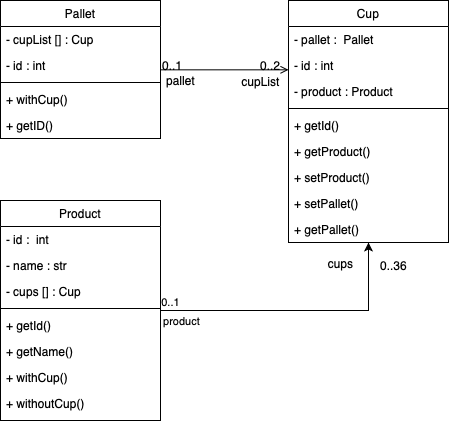
\includegraphics[width = \textwidth ]{Bilder/BeispielRefInt}
        \centering
\end{figure}

\newpage
\section{PySide6 und QuickQml 2.0}

Laut der Qt Wiki Website \cite{QtWikiHistory} wurde das Qt Framework geboren, als ihre Schöpfer Haavard Nord und
Eric Chambe-Eng im Sommer 1990 in Norwegen an einem GUI für eine Ultraschalldatenbank arbeiteten.
Die Software sollte damals in C++ implementiert auf Mac, Unix und Windows laufen.
Fünf Jahre später veröffentlichten Sie das erste Qt Framework unter dem Firmennamen Troll Tech.
Seitdem gewann das Framework immer mehr Popularität.
Im Jahr 2006 übernahm Nokia die Firma Troll Tech und verkaufte das Qt Project in den Jahren 2011 und 2012 erst teilweise,
dann vollständig an den Digia Konzern.
Seit 2014 ist Qt als Tochterunternehmen des Digia Konzerns unter dem Namen \glqq The Qt Company\grqq ein eigenständiges Unternehmen.

Das Qt Framework ist in C++ implementiert.
Die neue Software für die $\mu$Plant soll jedoch in Python implementiert werden.
Für diese Zwecke hat Qt u.A. das Framework PySide6 veröffentlicht, welches einen Wrapper für Python Projekte bietet.

GUI's können in PySide6 im Wesentlichen auf zwei Arten erstellt werden.
Eine Möglichkeit ist es, das GUI über Widgets\cite{pysideQtWidgets} zu erstellen, die direkt im Python Code implementiert werden können.
Die zweite Möglichkeit ist QtQuick \cite{pysideQtQuick} zu nutzen, bei dem das GUI in einer separaten QML Datei erstellt wird und
mittels einer \verb|QtQmlApplicationEngine| Klasse in das Programm eingebunden wird.

Für die Umsetzung eines MVC-Design Patterns empfiehlt sich die Verwendung von QtQuickQML.
Durch die Verwendung des Frameworks wird die konsequente Trennung zwischen Interface und Datenmodell erzwungen.
Veranschaulicht wird dies in Abb. \ref{fig:figure10}.
Die eigentlichen Daten (von Server oder Datei) werden in ein Datenmodell (Model) überführt.
Dieses Datenmodell ist ein beliebig komplexes Klassenkonstrukt, welches referenzielle Integrität aufbaut.
In Pyside6 muss dieses Datenmodell von der Basisklasse \verb|QAbstractModel| abgeleitet werden.
Beim Initialisierung der Anwendung wird eine Instanz dieser Klasse (oder einer abgeleiteten Klasse) erstellt und als
Root-context der \verb|QQmlApplicationEngine| registriert.
Somit ist das Datenmodell mit dem GUI verknüpft und kann unter seiner URI in jedem QML File angesprochen werden.
In einer QML Datei wird ein entsprechender QML Type, z.B. \verb|ListView|, welches eine einfache Liste erzeugt,
und dem Property \verb|model| die URI des Datenmodells zugewiesen.
Dadurch kennt das \verb|ListView| Objekt die Indices des Datenmodells und erhält beim Rendern der Liste nur die benötigten
Daten.\\
Jede weitere Aktion, die durch den Benutzer auf ein Listenelement ausgelöst wird, bezieht sich auf ein Delegate des Datenmodells.
Jede Änderung an dem Delegate wird zunächst gerendert und überprüft bevor das Datenmodell geändert wird.
Diese Basisfunktion kommt mit dem Qt Framework an sich und muss nicht implementiert werden.
Wie jedoch das Datenmodell mit den geänderten Daten umgeht oder ob die Änderung des Datenmodells automatisch ein Update
der Daten auf dem Server oder der Datei auslöst, muss vom Entwickler implementiert werden!\\
An ein Delegate sind je nach QmlType durch das Framework Signale gebunden.
Signale sind Teil des Signal/Slot Prinzips des Qt Framework \cite{pysideSignalSlot} und stellen die Funktion eines Events dar.
Durch die \verb|QmlApplicationEngine| sind innerhalb eines GUIs alle Root-context Elemente ansprechbar.
Wird ein Signal an beliebiger Stelle im GUI emittiert, kann es an jeder anderen Stelle als Event genutzt werden.
Dadurch muss man  in der Regel keine zusätzlichen Callbacks oder Lamda-Ausdrücke definieren.
Außerhalb des QML Contexts, z.B. in einer Python Klasse, muss das Signal der Klasse bekannt sein, indem das Signal an die Klasse
gebunden wird.
Eine Funktion die mit der Annotation \glqq Slot(str) \grqq versehen ist, wird als Slot behandelt und kann mit dem Signal
verknüpft werden, sodass diese bei Auftreten des Signals ausgeführt werden.
An Signale können Daten übergeben werden, die so in einem Slot weiterverarbeitet werden können.\\
\vspace{1cm}
In meiner Vorbereitung auf diese Arbeit hat sich eine intuitive Vorgehensweise entwickelt, die ich für die Implementierung
der Software empfehlen möchte:\\
\vspace{1cm}
Beim Initialisieren des Programms werden alle Datenmodelle (\verb|QAbstractModel| und abgeleitete Klassen), Controller
und Serviceklassen instanziert und als Root-context der \verb|QQmlApllicationEngine| gesetzt.
Siehe dazu das Beispiel \ref{exampleApp}.
Damit stehen sie dem Programmierer in jeder QML Datei der Anwendung zur verfügung.\\
In einer QML Datei können die Kontexte der QQmlEngine nun unter ihrer URI referenziert werden.
Dies ist in Beispiel \ref{exampleListview} gezeigt:\\
In dem QML Type \glqq ListView \grqq wird dem Property \verb|model| die URI des listModels aus \ref{exampleApp} zugewiesen.
Im weiteren Verlauf des Codes findet sich ein \verb|MouseArea| QML Type.
Wird in dem Bereich ein Klick mit linker Maustaste durchgeführt, wird das Signal \verb|onClicked| emittiert.
Innerhalb des \verb|MouseArea| Codes wird definiert, dass nach einem Mausklick die Funktion \verb|selectRow(message)|
aufgerufen wird. \verb|message| ist dabei der übergebene Parameter.
Das Beispiel braucht dabei keinerlei Importe anderer Klassen, was daran liegt, dass sowohl das DatenModell als
auch das Objekt der Controller Klasse als Ressource der QQmlEngine registriert wurden.\\
Im weiteren Verlauf des Codes wird ein QML Type \verb|Connections| erzeugt, bei dem das Signal des Controllers \verb|onRowClicked|
mit einer Funktion verbunden wird.
Innerhalb des \verb|Connections| Types wird in Javascript die Funktion definiert.
Zu beachten ist, dass im Controller selbst das Signal als \verb|RowClicked| definiert wird.
Innerhalb der QML Datei werden die Signale dann mit dem Präfix \glqq on \grqq erfasst.
Der Signalname wird als Name einer javascript - Funktion verwendet, die mit \verb|function| gekennzeichnet ist.
Der Code innerhalb des Funktionskörpers beschreibt dann die Funktionslogik in Javascript.
Im Fall des Beispiels wird ein bool'sches Property umgeschaltet, wenn die \verb|id| des Datenmodell - Delegates mit der
\verb|message| des Signals übereinstimmt.

\lstset{
    basicstyle=\small\ttfamily
}
\newpage
\lstinputlisting[language=Python,
        caption ={Beispiel einer einfachen App mittels PySide6. \small Zunächst wird eine Instanz der
Application-Klasse und der QmlEngine erzeugt. Danach werden Objekte eines Datenmodells und
eines Controllers erzeugt und als rootContext der QmlEngine registriert. Anschließend wird die QML Datei des Hauptfensters geladen,
was die App startet.}]
{Listings/Demo1.py}\label{exampleApp}

\lstinputlisting[language=xml,
caption ={Beispiel einer QML Datei\small Diese QML Datei erzeugt ListView QML Type, der zum Anzeigen der Daten
in einem ListModel verwendet wird. Innerhalb eines Rechtecks mit farbigem Rand werden in einem RowLayout Type die
Datensätze des Datenmodells gerendert und über die Funktionslogik von Signalen der QML Types und der Controllerklasse
farblioch markiert.}]{Listings/listviewExample.qml}\label{exampleListview}
\newpage

\begin{figure}
        \caption[Model-View Konzept mit zusätzlichem Controller und Service ]
        {\small Die Abbildung zeigt das in PySide6 verwendete Model-View Konzept, welches um einer Controllerklasse und
        einer Service Klasse erweitert wurde. }\label{fig:figure10}
        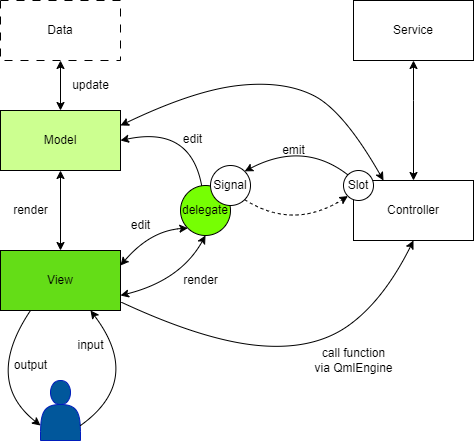
\includegraphics[width = \textwidth ]{Bilder/MVCS_Beispiel}
        \centering
\end{figure}

\newpage

Aus den Beispielen \ref{exampleApp} und \ref{exampleListview} lässt sich eine Systematik erkennen:
Die Daten sind hinter einem DatenModel geschützt und werden der View zur Verfügung gestellt.
Über die QML Dateien erfolgt die GUI Modellierung und Events werden mit dem Signal/Slot Prinzip behandelt.
Beliebige Ressourcen können als Teil der QmlEngine registriert werden, um Sie an anderer Stelle verfügbar zu machen.
Das künftige Programm soll jedoch auch Programmteile aufweisen, die nicht unbedingt mit den Daten oder dem GUI verknüpft sind.\\
Das sind beispielsweise die Kommunikationen über ModBus und dem ABB Industrieroboter oder das Übersetzen der Modbus Werte in
RAPID Befehle.
Diese Programmteile werden als Service Klassen bezeichnet.
Wenn sich der Programmcode auf ein GUI auswirkt, wird ein Controller gebraucht, der dieses Verhalten steuert.
Selbstverständlich könnten die Funktionen eines Controllers in den Service integriert werden.
Dies würde aber die Wartbarkeit und Erweiterbarkeit verschlechtern.
Nach der Systematik wie in \ref{fig:figure10} abgebildet, können beliebig viele Datenmodelle, GUI's, Controller und Services
parallel existieren ohne sich gegenseitig zu beeinflussen.\\
Als Nachteil kann angeführt werden, dass sich mit zunehmendem Kontextregister der QmlEngine die Performance des Programms
verschlechtern wird.
Bei dem eher gering erwarteten Funktionsumfang der zu erstellenden Software ist dies jedoch untergeordnet und könnte
durch das dezidierte Aufteilen der Funktionen in Threads reduziert werden.

\section{GUI - Konzeptionierung}

Die Hauptfunktion der Software war bisher das automatisierte Abarbeiten der Kommissionsaufträge, die über Modbus TCP/IP
von der Auftragsverwaltung der $\mu$Plant übergeben werden.
Während diese Funktion abläuft, macht der Benutzer höchstwahrscheinlich einen Soll-Ist-Vergleich zwischen dem GUI
und dem was er in der LZ sieht.
In Abb. \ref{fig:figure11} ist ein Entwurf dargestellt, der zeigt, welche Elemente im Automatikbetrieb sichtbar sein sollten:\\
Links ist die Andockstation des mobilen Roboters simuliert mit einem RFID Gerät darüber.
Die eingelesen Daten des RFID -Lesers könnten rechts daneben angezeigt werden.\\
Der Kommissioniertisch ist mit seinen beiden Plätzen \glqq K1 \grqq und \glqq K2 \grqq  daneben symbolisiert.\\
Die Visualisierung des Lagers nimmt den gesamten rechten Bildschirm ein.\\
Die Produktliste, wie sie in \ref{fig:figure} Bereich \glqq D\grqq dargestellt ist, kann entfallen.
Muss der Bediener ein Produkt an irgendeiner Stelle des Programms überschreiben, so wird ihm nicht mehr die Produkt ID
angezeigt, sondern direkt der Name.
Zusätzlich könnte die Produktliste als Neues Fenster auf Wunsch des Benutzers eingeblendet werden.
Zum Beispiel über die Toolbar.\\
Sämtliche Einstellungen wie Ip und Port der Kommunikationsschnittstellen sollen nur bei Bedarf angezeigt werden.
Dazu wird die Taste zum Aufrufen in der Toolbar platziert und die EInstellungen sollen in einem QML Type \verb|QDialog|
erfolgen.
Das hat den Vorteil, dass die Eingabe der Daten ohne viel Implementierung erfolgen kann ohne das Datenmodell zu ändern.
Eingegebene Daten müssen bestätigt werden und können auch wieder verworfen werden.\\
Die Bereiche \glqq E\grqq (Inventarliste) und \glqq F\grqq (Eventlog) aus Abb. \ref{fig:figure} müssen nicht
gleichzeitig sichtbar sein.
Sie können in einem Register integriert werden und mit dem QML Type \verb|StackView| oder einem Loader angezeigt werden.
Das Erscheinungsbild der beiden GUI Elemente kann aus der alten Software übernommen werden.\\
Als Drittes Register soll zusätzlich zum alten Startbildschirm eine Commission List (siehe Abb. \ref{fig:figure13}) hinzugefügt werden.
Sie soll eine Übersicht über die von der Auftragsverwaltung eingetroffenen Aufträge und ihren Status anzeigen.
Um manuelle Überschreibungen der Produkte und Cup IDs vorzunehmen, ist vorgesehen, dass ein Zahnrad-Symbol erscheint,
wenn man über dem entsprechenden Bereich den Mauszeiger hält (Hovering).
Bei Klick auf das Zahnrad-Symbol soll ein Objekt des QML Types \verb|QDialog| eingeblendet werden in dem die alten
Feldwerte angezeigt und editiert werden können, aber auch das Editieren verworfen werden kann.\\
\vspace{1cm}

Die Funktion des ehemaligen Controllers soll über die Toolbar aufgerufen werden.
Der Begriff an sich ist im Zusammenhang mit der neu konzipierten Software irreführend und wird daher verworfen.
Der stattdessen wird der Titel \glqq Manual Processing \grqq gewählt.
Hiermit sollen manuell Transportaufträge erzeugt werden wie \glqq Räume den Becher aus Lagerort L3a nach L6b \grqq.
Dies soll für jede sinnvolle Transportoperation möglich sein.
Bei Klick auf den entsprechenden Eintrag in der Toolbar könnte sich ein Fenster oder ein Dialog öffnen wie in
\ref{fig:figure12}.\\
Die so neu erzeugten Transportaufträge werden ebenfalls in der Commission List (siehe Abb. \ref{fig:figure13}) angezeigt.\\

\begin{figure}
        \caption[Mockup des Startbildschirms]
        {\small Die Abbildung zeigt wie der Startbildschirm aussehen könnte um die Funktion des Automatikbetriebs abzubilden:
        }\label{fig:figure11}
        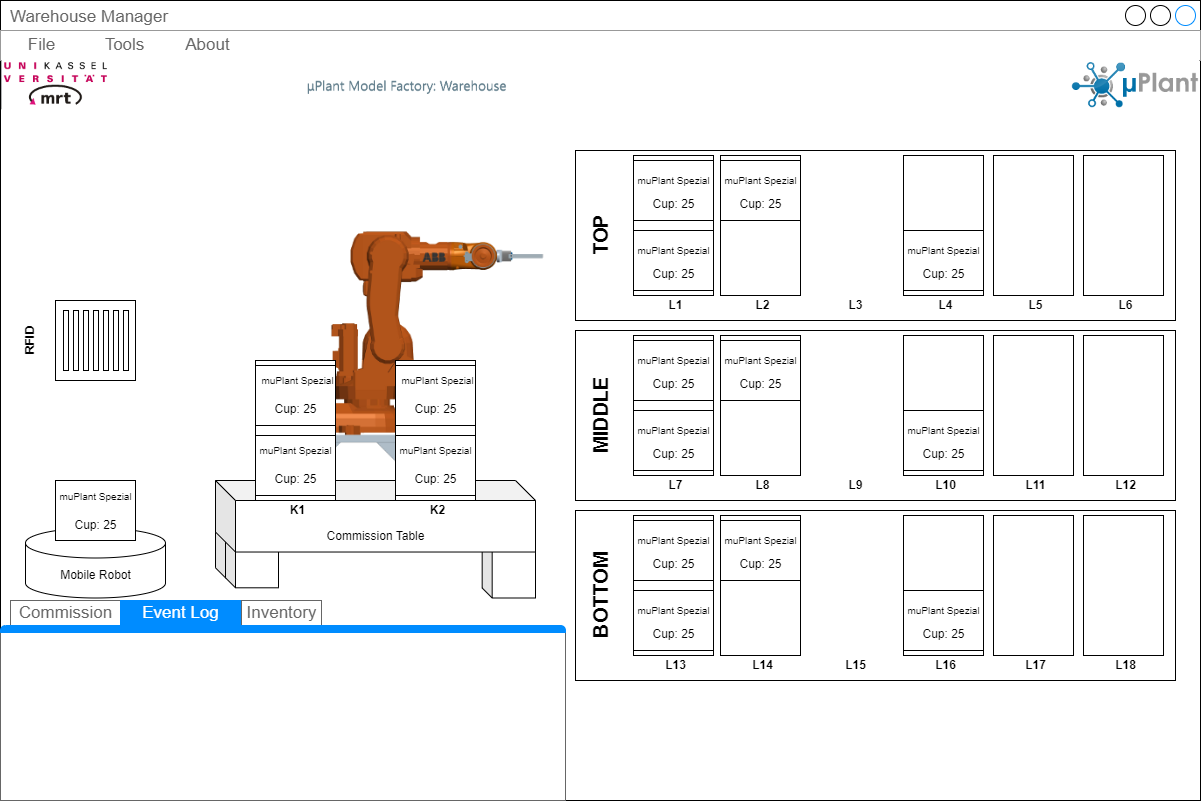
\includegraphics[width = \textwidth ]{Bilder/Mockup_Startbildschirm}
        \centering
\end{figure}

\begin{figure}
        \caption[Mockup des Menüs für die manuelle Lagersteuerung]
        {\small Die Abbildung zeigt, dass entweder ein Becher oder eine Palette (mit oder ohne Becher) vom Startort zum
        Zielort transportiert werden kann. Die Eingabe der Zielorte wird hier über zwei Dropdown Menüs realisiert.
        Das Mockup impliziert, dass bei Tätigung einer Eingabe eine Validierung der Eingaben erfolgt.
        }\label{fig:figure12}
        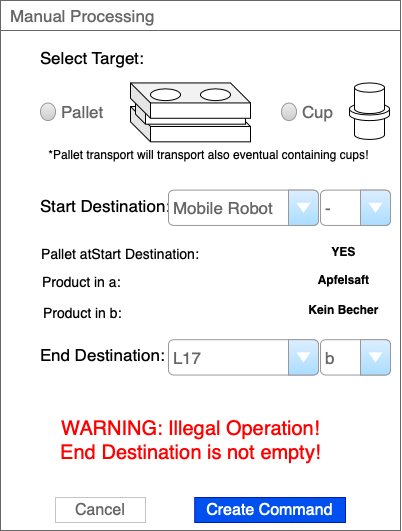
\includegraphics[height = 0.5\textwidth ]{Bilder/Mockup_ManualProcessing}
        \centering
\end{figure}

\begin{figure}
        \caption[Mockup der Commission List]
        {\small Die Abbildung zeigt, wie die Commission List aussehen könnte. Sie könnte als Tab in einem Register eingebunden werden.:
        }\label{fig:figure13}
        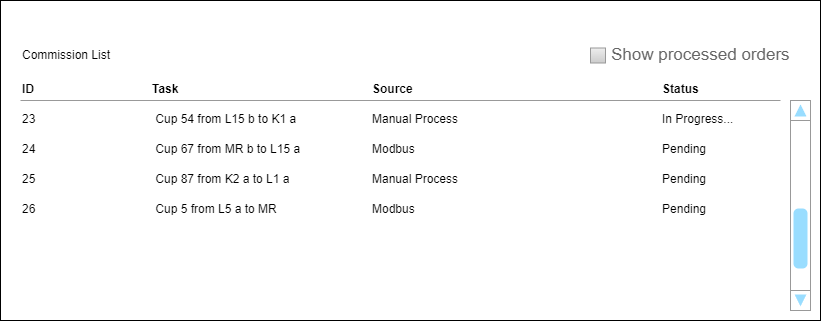
\includegraphics[width = \textwidth ]{Bilder/Mockup_CommissionList}
        \centering
\end{figure}
\vspace{1cm}
Das GUI des RFID Server Programms war sinnvoll und praktisch und kann so wie bisher umgesetzt werden.
Der Aufruf des Programms soll über die Toolbar implementiert werden.

\section{Konzepte zur Datenmodellierung}

Für die Modellierung der Daten wird das MVC Konzept angewandt und um Serviceklassen erweitert.
Bei der Anlieferung eines Bechers wird dieser in eine Palette gestellt und anschließend eingelagert.
Ein Objektdiagramm dieser Situation ist in Abb.\ref{fig:figure14} dargestellt.
Eine Palette kann keinen, einen oder zwei Becher beinhalten.
Die Becher in einer Liste zu speichern hat den Nachteil, dass man die Becher in der Palette als Listeneinträge verarbeiten muss
und der Slot als weitere Listenspalte geführt wird.
Die Becher als zwei separate Objekte in der Palette zu führen hat den Nachteil, dass zwei Orte abgefragt werden müssen.
Andererseits ist die Zuordnung des Bechers zum Slot dadurch inhärent.
Im Folgenden werden daher die Becher nicht als Liste, sondern als separate Feldwerte in der Palette geführt.\\
Abb. \ref{fig:figure14} zeigt auch, dass jedes Objekt der Klasse Palette und Cup ein Feld \verb|location| braucht.
Hier wird das Objekt gespeichert in welchem sich die Palette oder Becher gerade befindet.
Dies ist erforderlich um referenzielle Integrität zu gewährleisten und erleichtert die Implementierung der Controller,
wie eingangs in Kapitel \ref{PythonApp} beschrieben.
Aus dem Diagramm wird auch deutlich, dass zwsichen den Objekten der Klassen \verb|MobileRobot|, \verb|WorkBench| und
\verb|Inventory| keinerlei Assoziationen gibt.
Es wird also ein weiteres Objekt, z.B. ein InventoryController, gebraucht um aktiv Objekte von einem Lagerort zu einem Anderen
zu schreiben.\\
Als Ergebnis dieser Überlegungen leitet sich ein (Daten-)Klassendiagramm ab (Siehe Abb.\ref{fig:figure15}).\\
Weitere Daten des Programms werden erwartungsgemäß nur in den Service-Klassen (siehe Kapitel \ref{ControllerServices})
gebraucht.
Die werden daher auch dort gespeichert wo sie verarbeitet werden.
Immer wenn ein Service Zugriff auf das Datenmodell braucht, wird der entsprechende Controller diese Zugriffe verarbeiten.\\


\begin{figure}
        \caption[Objektdiagramm]
        {\small Die Abbildung zeigt ein Objektidiagramm aus Ablageorten für Paletten und Becher. Es ist ebenfalls
        ersichtlich, dass keine Verbindungslinien zwischen dem mobilen Roboter, dem Kommissioniertisch und dem Lager existieren.
        }\label{fig:figure14}
        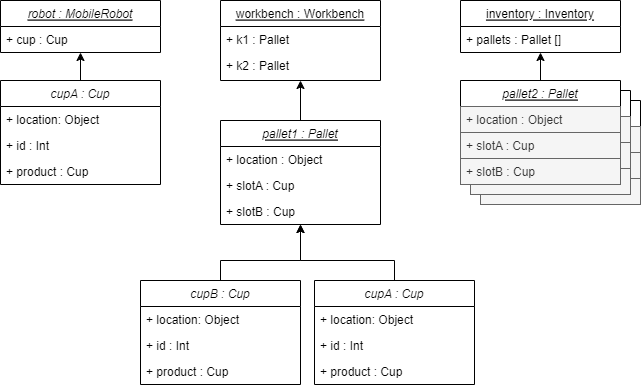
\includegraphics[width = \textwidth ]{Bilder/Objektdiagramm_PaletteCupStorage}
        \centering
\end{figure}

\begin{figure}
        \caption[Klassendiagramm Datenmodell ]
        {\small Klassendiagramm für die Datenstruktur der Software der Lagerverwaltung.
        }\label{fig:figure15}
        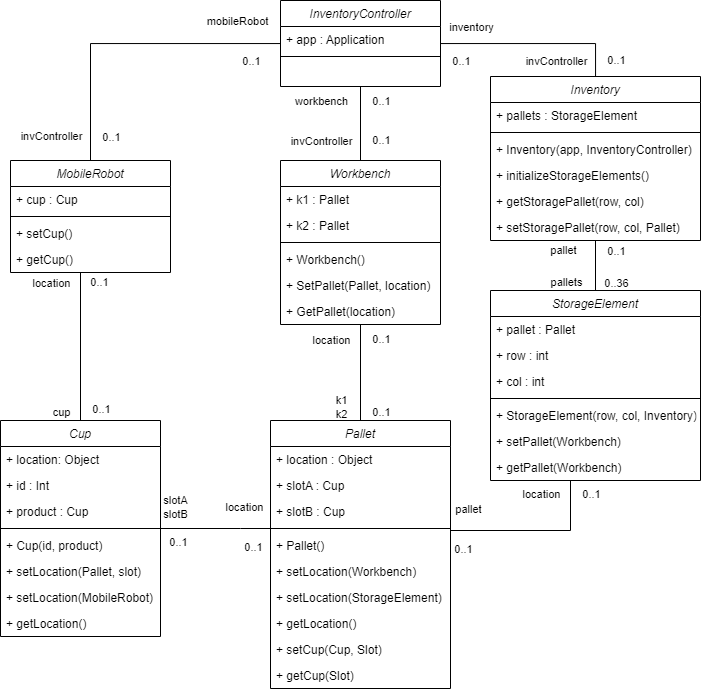
\includegraphics[width = \textwidth ]{Bilder/Klassendiagramm_Datenstruktur}
        \centering
\end{figure}


\section{Konzepte für Controller- und Serviceklassen}\label{ControllerServices}

Für die Kommunikation über Modbus TCP/IP, OPC UA, RFID und ABB Robotics wird jeweils eine eigene Serviceklassen angelegt,
wobei für Modbus TCP/IP  und OPC UA sowohl Client als auch Server gebraucht werden.
Das in \cite{LarsKistner2017} eingeführte Agentensystem wird ebenfalls als eigener Service implementiert.
Da die LZ nicht mit anderen Stationen kommunizieren muss, reicht die Implementierung des Clients.\\

Controller werden gebraucht um Schnittstellen zwischen Service und Daten oder zwischen Service und GUI zu implementieren.
Da Service und GUI im Allgemeinen getrennt sind, macht es am meisten Sinn, den Controller dem GUI zuzuordnen.
Controller wie \verb|EventlogController| machen Sinn, Controller wie \verb|ModBusController| eher weniger und implizieren
eine andere Aufgabe.

Eine besondere Rolle nimmt der \verb|InventoryController| ein.
Er muss zum Start des Programms das Inventar aus Dateien laden und damit das Datenmodell initialisieren.
Aus Gründen die in Kapitel \ref{Fehlerbehandlung} erörtert werden, sollte der Controller nach jeder vollständigen Änderung
des Datenmodells die Änderung einerseits in der Datei und andererseits in OPC UA sichern.

Eine Liste aller benötigter Service Klassen ist in Tab. \ref{tab:Services} aufgelistet.
Die Controller finden sich in Tab. \ref{tab:Controller}.


\begin{table}[h]
\centering
\caption{Benötigte Serviceklassen}
\begin{tabularx}{\textwidth}{|l|X|}
\hline
Klassenname & Beschreibung \\
\hline
Modbus Service & Implementiert die Modbus Kommuniktaion, sendet Modbus informationen an entsprechende Controller\\
\hline
OPC UA Service & Hält OPC UA Server und Client, organisiert Kommunikation zu anderen OPC UA entities\\
\hline
RFID Service & Erledigt alles was mit RFID zu tun hat\\
\hline
\end{tabularx}\label{tab:Services}
\end{table}


\begin{table}[h]
\centering
\caption{Werte der Klasse ModbusBaseAddress}
\begin{tabular}{|l|l|}
\hline
Klassenname & Beschreibung \\
\hline
InventoryController & Führt jede Operation bezüglich des Datenmodells aus \\
\hline
EventlogController & Erzeugt Meldungen für den Eventlog\\
\hline

\hline
\end{tabular}\label{tab:Controller}
\end{table}



\newpage
\section{Teilautomatisierte Code Dokumentation mit Sphinx}

Code-Dokumentation ist ein wichtiger Bestandteil jedes Softwareprojekts und dient dazu den Code anderen Entwicklern zugänglich zu machen.
Die Erstellung ist unter Umständen aufwändig, kann aber zumindest teilweise automatisiert werden.
Eine Möglichkeit besteht darin, das Paket Sphinx zu verwenden.
Sphinx ist ein Tool, das es Entwicklern ermöglicht, Dokumentationen in verschiedenen Formaten wie HTML, PDF und ePub
aus Kommentaren im Code des Python Projekts zu erstellen.
Dazu werden die in Python üblich Docstrings verwendet \cite{pepDocstrings}.\\
Das Paket kann über PyPi mit folgendem Kommando über die Eingabeaufforderung installiert werden:
\begin{lstlisting}
        pip install -U sphinx
\end{lstlisting}
\vspace{1cm}
Das Sphinx- Paket benutzt Themes um die Dokumentation grafisch darzustellen und zu strukturieren.
In Vorbereitung auf diese Arbeit habe ich mir das rtd-theme (Read the Docs \cite{RTD}) angeschaut und ausprobiert.
Es ist ein beliebtes Theme für Sphinx-Dokumentationen, da eine klare und übersichtliche Darstellung der Dokumentation
bietet und einfach zu verwenden ist. \\
Um das rtd-theme in einem Sphinx-Projekt zu verwenden, muss es zunächst installiert werden.
Dies kann über den Befehl
\begin{lstlisting}
        pip install sphinx_rtd_theme
\end{lstlisting}
erfolgen, dabei wird das Sphinx Paket auf die Version 6.4.1 angepasst.\\
\vspace{1cm}
Um Sphinx zu nutzen, muss es zunächst konfiguriert werden. Mit dem Kommando

\begin{lstlisting}[language = python]
        sphinx-quickstart
\end{lstlisting}
wird man Über die Konsole aufgefordert einige Optionen festzulegen mit denen die Dokumentation aufgesetzt wird.
Anschließend befinden sich in dem ausgewählten Ordner:
\begin{itemize}
        \item ein Makefile
        \item eine Datei \verb|modules.rst|
        \item eine Datei \verb|index.rst|
\end{itemize}

Index ist in der HTML -Version die Startseite.
Im RST-Format \cite{sphinxRST}kann die Seite gestaltet werden. \\
In der \verb|modules.rst| dagegen werden die Module aufgelistet, die dokumentiert werden sollen.
Nach der Installation des rtd-theme kann es in der Konfigurationsdatei von Sphinx aktiviert werden.
Dazu muss die Zeile \verb|html_theme = 'sphinx_rtd_theme'| in die Datei \verb|conf.py| eingefügt werden.
Sobald das Theme aktiviert ist, wird die Dokumentation im rtd-Theme angezeigt.\\

[Hier noch erklären wie sphinx verwendet wird falls Code aktualisiert oder gar neue Dateien hinhugefügt werden]
\subsection{Sphinx Erweiterungen}\label{subsec:sphinx-erweiterungen}

In der Konfigurationsdatei \verb|conf.py| habe ich folgende Zeile eingefügt:

\begin{lstlisting}[language = python,label={lst:sphinxExt}]
extensions = [
        'sphinx.ext.autodoc',
        'sphinx.ext.viewcode',
        'sphinx_copybutton']
\end{lstlisting}

\subsubsection{Autodoc}
Autodoc wird dazu verwendet um die Docstrings im Python-Code als Dokumentationstext zu erfassen.
Damit dies funktioniert muss ein Modul in der Datei \verb|modules.rst| mit folgendem Syntax hinzugefügt werden:
\begin{lstlisting}[language = python,label={lst:sphinxAutomodule}]
.. automodule:: src.cameraApplication.cameraProcessing
        :members:
\end{lstlisting}

Die Dateipfade der Module werden wie im Beispiel vom Makefile aus zur Python-Datei angegeben, jedoch ohne Dateierweiterung.
Docstrings in den Modulen werden direkt als HTML gerendert.
Inline-Kommentare werde nicht angezeigt.

\subsubsection{viewcode}

Um den Code des Moduls in dem HTML Dokument einzublenden wird die Erweiterung viewcode genutzt.
Unterhalb der Modulüberschrift im HTML-Dokumentwerden zunächst alle Docstrings gerendert.
Darunter erscheint nun ein grauer Bereich, in dem Python Code mit Farbformatierung angezeigt wird.
Es werden auch andere Sprachen erkannt, jedoch gibt es leider keine Option QML Code farblich formatiert
anzuzeigen.
QML Dateien werden im Allgemeinen von Autodoc nicht erkannt.
Die Einzige Option ist ein \verb|literalinclude| Befehl in der Datei \verb|modules.rst| wie z.B.:
\begin{lstlisting}[language = python,label={lst:sphinxQML}]
qml.main.qml
------------

The main QML-file creates the main application window.

.. literalinclude:: src/qml/main.qml
        :language: qml
\end{lstlisting}

Wie leicht zu erkennen werden Docstrings nicht erkannt und müssen daher manuell eingefügt werden.
Kommentare im Javascript-Syntax und Properties werden farblich hervorgehoben.
Insofern ist dies ein gangbarer Weg.

\subsubsection{sphinx\_copybutton}

Diese Erweiterung erleichtert dem Anwender oder Entwickler das Leben wenn durch die HTML Seite navigiert wird.
Werden Codes für die Kommandozeile in den rst Dateien angegeben, wie z.B.:
\begin{lstlisting}[label={lst:sphinxCodebutton}]
        .. code-block:: bash
                pip install -r requirements.txt
\end{lstlisting}
Dann wird im HTML Dokument im grau hinterlegten Bereich der den Code darstellt, ein Knopf gerendert,
der das Kommando per Click in den Zwischenspeicher kopiert.



\section{Sonstige Festlegungen}

\subsection{Virtual Environment}

Die Entwicklung der Software soll in einer virtuellen Entwicklungsumgebung (venv) stattfinden.
Alle benötigten Pakete werden dort installiert. \\

Die installierten Pakete werden nicht in das Git Repository gepusht. Stattdessen wird mit
\begin{lstlisting}[label={lst:freezeReq}]
        pip freeze > requirements.txt
\end{lstlisting}
Eine Textdatei mit allen verwendeten Bibliotheken erstellt.
Läd sich ein Benutzer das Repository herunter, können mit dem Befehl
\begin{lstlisting}[label={lst:installReq}]
        pip install -r requirements.txt
\end{lstlisting}
alle benötigten Pakete installiert werden, sodass das Projekt lauffähig kompiliert werden kann.
Der Nachteil ist, dass es im Aufgabenbereich des Entwicklers liegt, nicht verwendete Pakete zu deinstallieren,
sodass sie später nicht unbeabsichtigter Weise installiert werden.


\subsection{Verwendete Programme }

Nachfolgend werden alle verwendeten Programme und Software aufgelistet, die zur Erstellung der Software benutzt werden
\begin{itemize}
        \item PyCharm Comunity Edition von JetBrains wird zur Editierung von Code verwendet. Das betrifft nicht nur Python Code,
        sondern auch alle anderen Sprachen und Syntaxe exklusiv QML. Sogar zur Erstellung von LaTeX Dokumenten wird
        PyCharm mit dem PlugIn TeXiFy verwendet.
        \item Qt Creator kann für alle Qt kompatiblen Programmiersprachen verwendet werden. Es beinhaltet außerdem den
        Qt Designer, mit dem QML Dateien grafisch editiert werden können. Das Programm ist teilweise unbequem und umständlich,
        ist aber für QML in Python die beste Lösung um intuitiv Einstellungen an QML Types auszuprobieren.
        \item Visual Studio 2022 wird dazu verwendet den C\# Code der alten Software zu analysieren.
        Das PlugIn \glqq Class Designer \grqq wird dazu verwendet um die Projektmappen in Klassendiagramme darzustellen.
        \item Die Homepage Diagrams.net bietet eine gute Lösung um schnell Diagramme in UML und anderen Standards zu erstellen und
        in gewünschten Dateiformaten zu exportieren.
\end{itemize}
\cleardoublepage

\chapter{Analyse zur Fehlerbehandlung}\label{Fehlerbehandlung}

Fehler können systematischer oder sporadischer Natur sein.
Die effektive Fehlersuche und Fehlerbehebung ist ein wichtiger Bestandteil der Softwareentwicklung, der den Entwickler 
ständig begleitet. 

\subsection{Fehleridentifikation}

Syntaxfehler und Fehler in der Benutzung der Programmiersprache Python lassen sich in der Regel gut finden und beheben.
Der größte Teil wird bereits bei der Erstellung des Quellcodes erkannt und farblich markiert. 
Andere Fehler führen bei jedem Ausführen des Codes zu einem Ausnahmefehler, den der Interpreter erkennt und (meistens) eine brauchbare
Fehlermeldung in der Konsole ausgibt. 

Weitere Fehler sind oft in der Logik des Programms zu finden. Diese zu identifizieren ist in der Regel schwieriger.
Es ist jedoch möglich, nach dem Eingabe-Verarbeitung-Ausgabe Prinzip vorzugehen. 
Dabei bewertet man engmaschig die Eingabe und die Ausgabe und vergleicht Soll mit Ist. 

Eingaben können in einem Wertebereich möglich sein.
Hier muss der Entwickler alle erwartbaren Sonderfälle abdecken.
Für systematische Fehler können in der Softwareentwicklung Tests definiert werden, die das Programmverhalten 
für ein Spektrum an Eingaben überprüfen.
Die Ausgaben werden mit den erwarteten Ausgaben durch Assertions verglichen.
In Python ist dies beispielsweise mit dem Paket \verb|pytest| ( siehe \cite{pytestHP}) oder \verb|unittest| ( siehe \cite{unittestHP}) möglich.
Anhand einer kurzen Recherche beider Internetauftritte werde ich pytest verwenden.
Einerseits liefert pytest bei fehlgeschlagenen Tests eine ausführlichere Analysemeldung, adererseits wird pytest von Qt empfohlen.
Mit pytest lassen sich aber nur Python Module testen.

Für einen GUI Test muss das \verb|QtTest| Framework verwendet werden.
Leider lässt sich zu diesem Paket keine umfangreiche Dokumentation. 
Ich habe versucht dieses Framework zusammen mit dem Qt Creator zu benutzen. 
Entweder erhielt ich Fehlermdleungen, die ich nicht mit meinem Code in Verbindung bringen konnte 
oder das Ausführen des Programms ignorierte die geschriebenen Tests.
Dies bewegt mich zu der Empfehlung von diesem Framework ohne weitere Updates und Dokumentation seitens Qt abzusehen.

Sporadische Fehler können nicht unbedingt vorhergesehen werden. 
Sie rühren meistens aus einer unerwarteten Kombination von Eigaben die selten auftritt oder durch einen Fehler in einerm eingebundenen Dienst. 
Eine gut dokumentierte API weist auf Fehlermöglichkeiten hin und gibt Hinweise zur Fehlerbehandlung.
Die erwarteten Quellen sind Eingabefehler und Kommunikationsfehler.

\subsection{Erkennung fehlerhafter Benutzereingaben}

Werden im Programm falsche Daten eingegeben eingelesen, soll dies, soweit wie möglich, entdeckt und abgefangen werden.
Die Tabelle \ref{tab:Benutzereingaben} listet alle erwarteten Benutzereingaben und mögliche Methoden die Benutzereingaben
zu validieren.

\begin{table}[h]
\centering
\caption{Benutzerinageben, mögliche Fehler und ihre Erkennung}
\begin{tabularx}{\textwidth}{|l|p{2cm}|p{2cm}|X|}
\hline
Art & Typ & Wertebereich & Fehlererkennung \\
\hline
IP Adresse & Formatierter String aus Integers & 0 \ldots 255 bzw. 0 \ldots 9 & Gültigkeitsprüfung bei Dateneingabe, Validierung bei Verbindungsaufbau\\
\hline
IP Port & Integer & 0\ldots65536 & Wertebereich bei Dateneingabe, Validierung bei Verbindungsaufbau\\
\hline
Produkt ID & Integer & 0\ldots99 & Eingabe anhand Dropdown Menü mit Anzeige des Produktnamens beschränkt Wertebereich auf zulässige Werte. Validierung nur im Softwarebetrieb durch Soll-Ist Abgleich.\\
\hline
Becher ID & Integer & 0\ldots99 & Eingabe kann nicht auf gültigen Wertebereich beschränkt werden. Soll-Ist-Vergleich mittels RFID ist möglich.\\
\hline
Palette & Bool & True / False & Abgleich mit Anwesenheit von Bechern, arUco Marker Erkennung mittels Kamera\\
\hline
\end{tabularx}\label{tab:Benutzereingaben}
\end{table}



Wenn manuell Transportaufträge eingegeben werden, kann es zu Konflikten kommen.
Z.B. Könnte im Abholort kein Becher oder keine Palette sein.
Umgekehrt könnte am Abstellort eine Palette oder Becher stehen.
Für diese Problematiken können :
\begin{itemize}
    \item Inventardaten zur Überprüfung herangezogen werden
    \item Kameragestützte Validierungsprozesse in Kapitel \ref{Kap5} Entworfen werden.
\end{itemize}
\cleardoublepage

\chapter{Ideensammlung zu kameragestützten Validierungsprozessen in der Lagerverwaltung}\label{Kap5}

Die neue Softwareanwendung soll die Möglichkeit bieten, das Inventar der Lagerzelle automatisiert zu überprüfen. 
Zu diesem Zweck sollen kameragestützzte Validierungsprozesse implementiert und untersucht werden. 
Dieses Kapitel soll dafür ein Konzept entwickeln und offensichtliche Anforderungen an die Kamera ableiten.

\subsection {Konzepte}

Die Lagerzelle beinhaltet ein Regal und einen Kommissionier-Tisch, der Paletten und Becher mit ggf. Produkten enthält.
Produkte werden dabei durch Wasser, die mit farbigen Kugeln vermengt sind, simuliert.
Ein Produkt wird von einem mobilen Roboter in einem Becher angeliefert. Anschließend wird es von dem Roboterarm in das Regal geräumt und verbleibt dort bis zu seiner Auslieferung.
Die Softwareanwendung merkt sich den Inventarbestand und seine Position im Regal.
Eine Manipulation des Inventars ist durch eine Person jederzeit möglich.
Ebenso eine Fehleingabe. 

Für eine kameragestützte Inventur gibt es somit zwei Usecases: 
Zum einen könnte eine Inventur auf Anforderung eines Benutzers durchgeführt werden um einen Soll-Ist Abgleich des realen Inventars mit 
dem gespeicherten Stand der Softwareanwendung vorzunehmen. 
Zum Beispiel, weil nicht mehr sichergestellt werden kann, dass die Bestandsdaten korrekt sind.
Zum anderen können die Produkte und Becher bei Anlieferung und Auslieferung automatisch verifiziert und Diskrepanzen dem Benutzer angezeigt werden.
Wenn die kameragestützte Inventur mittels einer Kamera auf dem Greifer durchgeführt wird, kann die Lagerzelle in dieser Zeit keine Transportaufträge bearbeiten.
Um einen Lagerort zu verifizieren, muss der Greifer vor die Palette fahren, kontrollieren, dass die Palette an Ort und Stelle ist, und den vorderen Becher prüfen. 
Anschließend muss der Greifer die Palette aus dem Regal holen und auf den Kommissionier-Tisch stellen.
Erst jetzt kann der Greifer den hinteren Becher prüfen und die Palette wieder in das Regal stellen.

Wenn der Roboterarm aus einer schnellen Bewegung heraus für eine Aufnahme stoppt, ist zu erwarten, dass aufgrund von Schwingungen nicht direkt mit der Bildaufnahme begonnen werden.
Eine Bildaufnahme an sich kann ebenfalls bis zu 5 Sekunden dauern. 
Wenn man überschlägt, dass für die Anfahrt, Auslagern und Einlagern je 5 Sekunden benötigt werden (was eine eher optimistische Schätzung ist), dauert eine Inventur pro Lagerort 25 Sekunden.
Bei 18 Paletten, ist die Lagerzelle somit für 7,5 Minuten blockiert.
Soll dazu noch das Produkt bewertet werden, muss der Greifer, nach dem die Palette auf dem Kommissionier-Tisch abgestellt wurde, von oben in den Bescher schauen und die Farben der drei 
Kugeln erkennen.
Eine andere Möglichkeit ist, eine Übersichtskamera zu verwenden. 
Diese ist an einem Ort in der Lagerzelle montiert, von dem aus alle Lagerorte, möglichst gut, überblickt werden können.
So kann während die Lagerzelle in Betrieb ist, das Inventar überprüft werden.
Bedingung dafür ist, dass die optischen Marker gut sichtbar und hoch genug aufgelöst sind.
Selbst wenn nicht alle optischen Marker von der Übersichtskamera erkannt werden können, so können dennoch von den erkannten Markern Rückschlüsse auf die Gültigkeit des Inventars gezogen werden. 
Oder aber die Daten, die mit der Übersichtskamera gewonnen werden, reduzieren die Zeit, die für die Inventur mit der Greifer-Kamera benötigt wird.


\subsection {Abgeleitete Anforderungen an die Kamera}

Für die Kameras, die für die kameragestützte Inventur verwendet werden, lassen sich aus dem Konzept Anforderungen ableiten. 
Der Greifer ist hoch beweglich und bietet aufgrund seiner Kinematik wenig Platz für eine Kamera. 
Die Kamera kann daher nur direkt auf dem Greifer befestigt werden. 
Ist ein Becher im Greifer ergibt sich daraus eine sehr kurze Distanz zwischen dem Kamerasensor und dem optischen Marker (etwa 30mm, je nach Kamera).
Die in \cite[Sebastian Hüblers Arbeit]{Hübler2019} verwendete $\mu$Eye Kamera konnte mit dem Abstand gut umgehen, wenngleich die optische Marker nicht mehr scharf sichtbar waren.
Leider ist diese Kamera defekt und es bedarf daher einer Neuanschaffung. 

An die Auflösung der Kamera auf dem Greifer gibt es keine besonderen Anforderungen, da die Marker erwartungsgemäß beinahe den gesamten Bildbereich einnehmen werden. 
Soll das Produkt erkannt werden, muss die Kamera einen RGB-Sensor haben.
Am Arm des Greifers ist bereits eine USB 2.0 Leitung verlegt, die benutzt werden soll. 

Eine Übersichtskamera wird für die größtmögliche Übersicht in eine der oberen Raumecken der Lagerzelle montiert.
Von dort aus, ist die Mitte des Regals etwa 3m entfernt. 
Bei einem arUco Marker mit einer 6x6 Binärmatrix und einer Kantenlänge von ca. 30mm, ist ein Bit etwa 3x3mm groß.
Da das Regal nicht den gesamten Bildbereich einnimmt, ist je nach Apertur der Kamera eine Auflösung von mehr als 20MP nötig. 
Zu dieser Auffassung komme ich nach Rücksprache mit dem Kamerahersteller IDS. 

Eine Kamera in der Raumecke muss sowohl eine Datenverbindung als auch eine Stromversorgung zur Verfügung gestellt bekommen.
Hochauflösende Kameras sind in der Regel mit GigE verfügbar und können über PoE mit Spannung versorgt werden. 
Eine Kamera, die beides erfüllt, spart die Verlegung einer weiteren Leitung. 


\subsection{Anforderungen an die Softwareanwendung}

Die Softwareschnittstelle der Kameras muss entweder OpenCV kompatibel sein oder eine Python-API bereitstellen.
Da einzelne Bilder verarbeitet werden sollen, ist eine hohe Bildrate nicht notwendig.
Zunächst wird mit der Übersichtkamera eine Bildaufnahme gemacht und daraus mit den Methoden der Bildverarbeitung alle optischen Marker erkannt - wo möglich.
Ein Vergleich mit dem Datenmodell ergibt die Positionen, bei denen eine Erkennung nicht funktionierte.
Für diese Positionen muss anschließend der Greifer die Inventurschritte übernehmen.
Erreicht der Roboter einen Ort von dem aus ein Bild aufgenommen werden soll, so muss er an die Softwareanwendung ein Signal senden, welches
der \verb|ABBController| verarbeitet und eine Bildaufnahme auslöst.
Während der Implementierung ist zu untersuchen, ob die Signale des Roboters Informationen über die Position enthalten müssen, oder ob die Position des Greifers aus dem Algorithmus abgeleitet werden kann.
Anschließend muss der Erkennungsalgorithmus ausgeführt werden.
Diese Schritte werden wiederholt, bis alle Lagerorte überprüft wurden.  
Sind die Inventurdaten vollständig, müssen die Daten mit den gespeicherten Daten verglichen werden.
Aus den Bildern und den daraus erkannten Daten muss eine Übersichtsansicht erstellt und angezeigt werden. 
Hier soll der Soll/Ist-Vergleich veranschaulicht werden. 
Bei Diskrepanzen soll ein Benutzer die Möglichkeit haben die Daten vereinzelt zu korrigieren, die Übernahme zu bestätigen oder zu verwerfen.



\cleardoublepage

% !TeX spellcheck = de_DE
\chapter{Zusammenfassung und Ausblick}

In dieser Arbeit wurde ein breiter Themenbogen gespannt, der von der Analyse der Architektur und Funktion einer C$\#$ / .NET Softwareanwendung bis zur
Konzeptionierung einer neuen Anwendung in Python mit Qt reicht.
In der Auseinandersetzung der Programmiersprachen C$\#$ und Python wurden ihre Unterschiede diskutiert und aufgezeigt, dass eine Portierung 1:1 nicht möglich ist.
Eher handelt es sich dabei um eine Neuentwicklung, die die Funktionen der alten Software übernimmt und um den neuen Kommunikationsstandard OPC UA erweitert.

Mit Augenmerk auf das GUI, wurden wesentliche Informationen und ihre Visualisierung diskutiert und Entwürfe für die neue Anwendung vorgestellt. 
Eine Analyse hat gezeigt, dass der Hauptbildschirm aufgeräumt werden kann, sodass der Hauptbildschirms den Lagerprozess und die Lager-Visualisierung
fokussiert. 
Diejenigen Informationen, die dabei nicht mehr angezeigt werden, können dabei in einem Dialog oder einem neuen Fenster angezeigt werden.
Der Dienst zur manuellen Lagerbedienung wird, genau wie der RFID-Server, als Plugin ausgeführt.

Aspekte der Implementierung wurden diskutiert und veranschaulicht, wie der Aufbau der neuen Anwendung unter Berücksichtigung des MVVC-Konzepts gelingen kann. 
Es wurde detailliert auf die Datenmodellierung eingegangen und die Vorteile der Referenziellen Integrität diskutiert und an Beispielen gezeigt.

Für die Zukunft wurde festgelegt, dass die Weiterentwicklung und Wartung der Anwendung bereits bei der Entwicklung der neuen Anwendung berücksichtigt werden soll. 
Zu dem Zweck werden die einzelnen Controller- und Serviceklassen auf eine enge Kernfunktion beschränkt. 
Die Verwendung der in Python eingebetteten Doc-Strings soll verwendet werden, um mit dem Paket Sphinx eine automatisierte Dokumentation zu erstellen.
Es wurden zudem zwei andere Pakete vorgestellt und diskutiert, mit denen Python-Module getestet werden können, um schnell die Konsistenz des Datenmodells zu überprüfen.
Diese beiden Aspekte sollen es anderen Personen erheblich erleichtern sich in die neue Anwendung einzuarbeiten, um sie zu warten oder zu erweitern.

Der Schwerpunkt des Ausblicks liegt auf der Ideensammlung für kameragestützte Validierungsprozesse in der Lagerzelle.
Es wurden zwei Usecases vorgestellt und Aspekte des Ablaufs diskutiert.
Aus den Ideen wurden Anforderungen an die Kameras und die Implementierung der Software abgeleitet.

%%% Local Variables:
%%% mode: latex
%%% TeX-master: "../MRT-Bericht2020"
%%% End:

\cleardoublepage

% --------------------------------------------------------------------------
% Anhang (WENN NÖTIG)
% --------------------------------------------------------------------------
\appendix
%\pagenumbering{roman}\setcounter{page}{1}
\pagenumbering{Roman}\setcounter{page}{\value{SeitenzahlSpeicher}}

% !TeX spellcheck = de_DE

\chapter{Dies ist der erste Anhang}

Hier Text einfügen.

\cleardoublepage

% --------------------------------------------------------------------------
% Literatur (IMMER)
% --------------------------------------------------------------------------
\addcontentsline{toc}{chapter}{Literaturverzeichnis}

%\bibliographystyle{Literatur/IEEEtran}
%\bibliographystyle{Literatur/IEEEtranS}
%%Deutsch (Groß/kleinschreibung)
\bibliographystyle{Literatur/IEEEtranGER}
%%Deutsch (Groß/kleinschreibung) + DOI
%\bibliographystyle{Literatur/IEEEtranGERdoi}
\bibliography{Literatur/Semesterarbeit}
	
% --------------------------------------------------------------------------
% Ende des Dokuments
% --------------------------------------------------------------------------
\end{document}

%%% Local Variables:
%%% mode: latex
%%% TeX-master: t
%%% End:
